%%%%%%%%%%%%%%%%%%%%%%%%%%%%%%%%%%%%%%%%%%%%%%%%%%%%%%%%%%%%%%%%%%%%
%PLANTILLA DE INFORMES V 1.1
%
% REQUISITO: IMPORTE EL LOGO DE LA USM CON EL NOMBRE "logousm.png"
% IMPORTE IMAGENES DE MODULOS, EXTRAER DEL WORD
%
% Material de referencia de proposito general:
% https://users.dcc.uchile.cl/~jbarrios/latex/
% http://mate.dm.uba.ar/~pdenapo/tutorial-latex/node2.html
% http://tiburondealambre.blogspot.cl/2012/01/referencias-imagenes-y-tablas-en-latex.html
% BIBLIOGRAFIA: http://logistica.fime.uanl.mx/miguel/docs/BibTeX.pdf
%
% Tratar ecuaciones en latex(muy util):
% https://ondiz.github.io/cursoLatex/Contenido/05.Ecuaciones.html
%
% detector de cosas dibujadas latex: http://detexify.kirelabs.org/classify.html
%
%%%%%%%%%%%%%%%%%%%%%%%%%%%%%%%%%%%%%%%%%%%%%%%%%%%%%%%%%%%%%%%%%%%%%%%

\renewcommand{\w}{\omega}
%----------------------PAQUETES---------------------------%
% No es necesario tocar nada de esto

\documentclass[12pt,a4paper]{article} % tipo de documento, formato

\usepackage[utf8]{inputenc}    % con tildes
\usepackage[spanish]{babel}    % arreglar problemas

\usepackage[framed,numbered,final]{mcode} %%MATLAB
\usepackage{listings}   % Permite incorporar código con d


\usepackage{graphicx} % paquete de tratado de imagenes/figuras
\usepackage{tipa} % para <
\usepackage{amssymb} % para >=

% paquete extra para ocupar [H] (obliga a que la imagen con graphicx
% se quede donde se realizó el llamado)
\usepackage{float}

% CARGAMOS 3 PAQUETES
% (AMS Math), que mejora el comportamiento y el aspecto de las ecuaciones. 
% Nos permite, por ejemplo, añadir un asterisco en el entorno equation para crear
% ecuaciones sin numerar.
%(AMS Theorem), que define los entornos teorema y demostración.
%(AMS Symbol), que carga a su vez amsfonts e incluye una colección 
%de símbolos matemáticos.
\usepackage{amsmath, amsthm, amssymb} 

\usepackage{enumerate} %permite enumerar de varias formas

\usepackage{multirow, array} % para las tablas

% construccion de un nuevo comando
\usepackage{lipsum}% http://ctan.org/pkg/lipsum
\usepackage{xcolor}% http://ctan.org/pkg/xcolor
\usepackage{xparse}% http://ctan.org/pkg/xparse
\NewDocumentCommand{\myrule}{O{1pt} O{2pt} O{black}}{%
  \par\nobreak % don't break a page here
  \kern\the\prevdepth % don't take into account the depth of the preceding line
  \kern#2 % space before the rule
  {\color{#3}\hrule height #1 width\hsize} % the rule
  \kern#2 % space after the rule
  \nointerlineskip % no additional space after the rule
}

%acomoda margenes y tipografia para que quede mas bonito
\usepackage{geometry}
\geometry{
	paper=a4paper, % Change to letterpaper for US letter
	inner=3cm, % Inner margin
	outer=3cm, % Outer margin
	bindingoffset=.5cm, % Binding offset
	top=2cm, % Top margin
	bottom=2cm, % Bottom margin
	%showframe, % Uncomment to show how the type block is set on the page
}


%---------PORTADA, TABLA DE CONTENIOS Y FIGURAS--------------%
%Esto será la portada. Solo hay que cambiar los textos
\begin{document}

\begin{titlepage}
\begin{center}
\textbf{\LARGE Universidad Técnica Federico Santa}\\[0.25cm]
\textbf{\LARGE María}\\[0.5cm]
\textbf{\large DEPARTAMENTO DE INGENIERÍA ELECTRONICA}\\[0.2cm]
\vspace{20pt}

\includegraphics{logousm.png}\\[1cm]

\par
\vspace{15pt}
\textbf{\Large ELO 314 - Laboratorio de procesamiento Digital de Señales}\\
\vspace{15pt}
\myrule[1pt][7pt]
\textbf{\LARGE Transformada Discreta de Fourier en MatLab}\\[0.25cm]
\vspace{15pt}
\textbf{\large  }\\
\myrule[1pt][7pt]
\vspace{55pt}
\textbf{\large Estudiante \hspace{75pt} ROL}\\
    \hspace{0pt}Rodrigo Graves\hspace{80pt} 201621009-1 \\
     Ricardo Mardones      \hspace{60pt} 201621036-9 \\
   


\vspace{30pt}
\textbf{\large Paralelo: \hspace{30pt} 1}\\

\vspace{35pt}
\textbf {\large Profesor}\\[0.2cm]
\Large { Gonzalo Carrasco}\\[0.1cm]
\textbf {\large Ayudante}\\[0.2cm]
\Large {Jaime Guzmán}\\[0.1cm]
\end{center}

\par
\vfill
\begin{center}
\textbf{Fecha : \today}\\
\end{center}

\end{titlepage}


%-------------Lista de figuras y tablas----------%
\tableofcontents % Hace el índice de contenidos. Latex organiza todo solito
\clearpage

\listoffigures %lista de figuras
\clearpage

\listoftables
\clearpage


\newpage
\section{Cálculo de la DFT para señales simples}
Para esta sección se consideran las señales $x_1(t) = \sin{(\omega t)}$, $x_2(t) = \cos{(\omega t)}$, ambas con frecuencia 100 Hz y muestreadas a $f_s = 5~kHz$ durante $100~ms$.

\begin{enumerate}
    \item Se pide obtener expresiones analíticas para las DTFT de las señales muestreadas $x_1[n],~ x_2[n]$, considerando duración infinita y los 100 ms.
    
    \textbf{DTFT de $x_1(n)$ de duración infinita:}
    
    En primer lugar se obtiene la versión muestreada de la señal en el dominio temporal:
    $$ x_1[n] = \sin{(2\pi f/f_s~n)} =  \sin{(0.04\pi n)} = \sin{(\omega_0 n)}$$
    
    Luego la DTFT está dada por:
\begin{align*}
    X_1(\omega) &= \sum_{n=-\infty}^{\infty}x_1[n]e^{-j\omega n}\\
    &= \sum_{n=-\infty}^{\infty}\sin{(\omega_0 n)}e^{-j\omega n}\\
    &= \sum_{n=-\infty}^{\infty}\left(\dfrac{e^{j\omega_0n} - e^{-j\omega_0n} }{2j}\right)e^{-j\omega n}\\
    &= \dfrac{1}{2j}\left(\sum_{n=-\infty}^{\infty}e^{j\omega _0n}e^{-j\omega n} - \sum_{n=-\infty}^{\infty}e^{-j\omega_0 n}e^{-j\omega n}\right)\\
    &= \dfrac{1}{2j}\left(2\pi\delta(\w-\w_0) - 2\pi\delta(\w+\w_0)\right)\\
    &= \dfrac{\pi\delta(\w-\w_0) - \pi\delta(\w+\w_0)}{j}\\
\end{align*}

    Cabe destacar que la expresión obtenida considera $\w \in [-\pi, \pi] $, si se desea para todo $\w$ debe considerarse periodicidad de periodo $2\pi$ del espectro en frecuencia.
    
    \textbf{DTFT de $x_2(n)$ de duración infinita:}
    
    Se obtiene la versión muestreada de la señal en el dominio temporal:
    $$ x_2[n] = \cos{(2\pi f/f_s~n)} =  \cos{(0.04\pi n)} = \cos{(\omega_0 n)}$$
    
    Luego la DTFT está dada por:
\begin{align*}
    X_2(\omega) &= \sum_{n=-\infty}^{\infty}x_2[n]e^{-j\omega n}\\
    &= \sum_{n=-\infty}^{\infty}\cos{(\omega_0 n)}e^{-j\omega n}\\
    &= \sum_{n=-\infty}^{\infty}\left(\dfrac{e^{j\omega_0n} + e^{-j\omega_0n} }{2}\right)e^{-j\omega n}\\
    &= \dfrac{1}{2}\left(\sum_{n=-\infty}^{\infty}e^{j\omega _0n}e^{-j\omega n} + \sum_{n=-\infty}^{\infty}e^{-j\omega_0 n}e^{-j\omega n}\right)\\
    &= \dfrac{1}{2}\left(2\pi\delta(\w-\w_0) + 2\pi\delta(\w+\w_0)\right)\\
    &= \pi\delta(\w-\w_0) + \pi\delta(\w+\w_0)\\
\end{align*}

    Cabe destacar que la expresión obtenida considera $\w \in [-\pi, \pi] $, si se desea para todo $\w$ debe considerarse periodicidad de periodo $2\pi$ del espectro en frecuencia.
    
    \textbf{DTFT de $x_1[n]$:}
    
    Debido a que $x_1[n]$ corresponde a la señal de duración infinita multiplicada por una ventana cuadrada, se obtiene su DTFT como la convolución de el espectro de la señal de duración infinita y el espectro de la ventana cuadrada $W(e^{j\w})$
    
    El espectro de la ventana está dado por:
    $$W(e^{j\omega}) = e^{-j\omega(N-1)/2}\dfrac{\sin{(\omega N}/2)}{sin(\w/2)}$$
    donde $N=500$ ya que la ventana de 100 ms es de 500 muestras.
    
    Luego el espectro de la señal enventanada está dado por:
    \begin{align*}
       X_1^{(w)}(\w) &= X_1(\w) \ast W(e^{j\omega})\\
       &= \left(\dfrac{\pi\delta(\w-\w_0) - \pi\delta(\w+\w_0)}{j}\right)\ast W(e^{j\omega})\\
       &=\dfrac{\pi W(e^{\w-\w_0}) - \pi W(e^{\w-\w_0})}{j}
    \end{align*}
    
    Lo cual permite bosquejar el espectro, pues aparecen sincs periódicas en las frecuencias $\pm \w_0$
    
    \textbf{DTFT de $x_2[n]$:}
    
    Similar al caso anterior, se obtiene su DTFT como la convolución de el espectro de la señal de duración infinita y el espectro de la ventana cuadrada $W(e^{j\w})$. 
    
    Luego el espectro de la señal enventanada está dado por:
    \begin{align*}
       X_2^{(w)}(\w) &= X_2(\w) \ast W(e^{j\omega})\\
       &= (\pi\delta(\w-\w_0) + \pi\delta(\w+\w_0))\ast W(e^{j\omega})\\
       &=\pi W(e^{\w-\w_0}) + \pi W(e^{\w-\w_0})
    \end{align*}
    
    Lo cual claramente permite bosquejar el espectro, pues aparecen sincs periódicas en las frecuencias $\pm \w_0$
    
    
    
    
    %%%%%%%%%%%%%%%%%%%%%%%%%%%%%%%%%%%%%%%%%%%%%%%%%
    
    \item Se obtiene mediante el comando \texttt{fft} de MATLAB, con un N = 4096 la magnitud de la DFT para las dos señales  analizadas en el inciso anterior, $x_1 = sin(\omega t)$ y $x_2 = cos(\omega t)$, los resultados se graficaron en los rangos $[-\frac{fs}{2},\frac{fs}{2}]$  y $[0,\frac{fs}{2}]$. Estas gráficas se muestran en las figuras \ref{fs-medios} y \ref{cero-fs-medio}
    
    
    \begin{figure}[H]
        \centering
        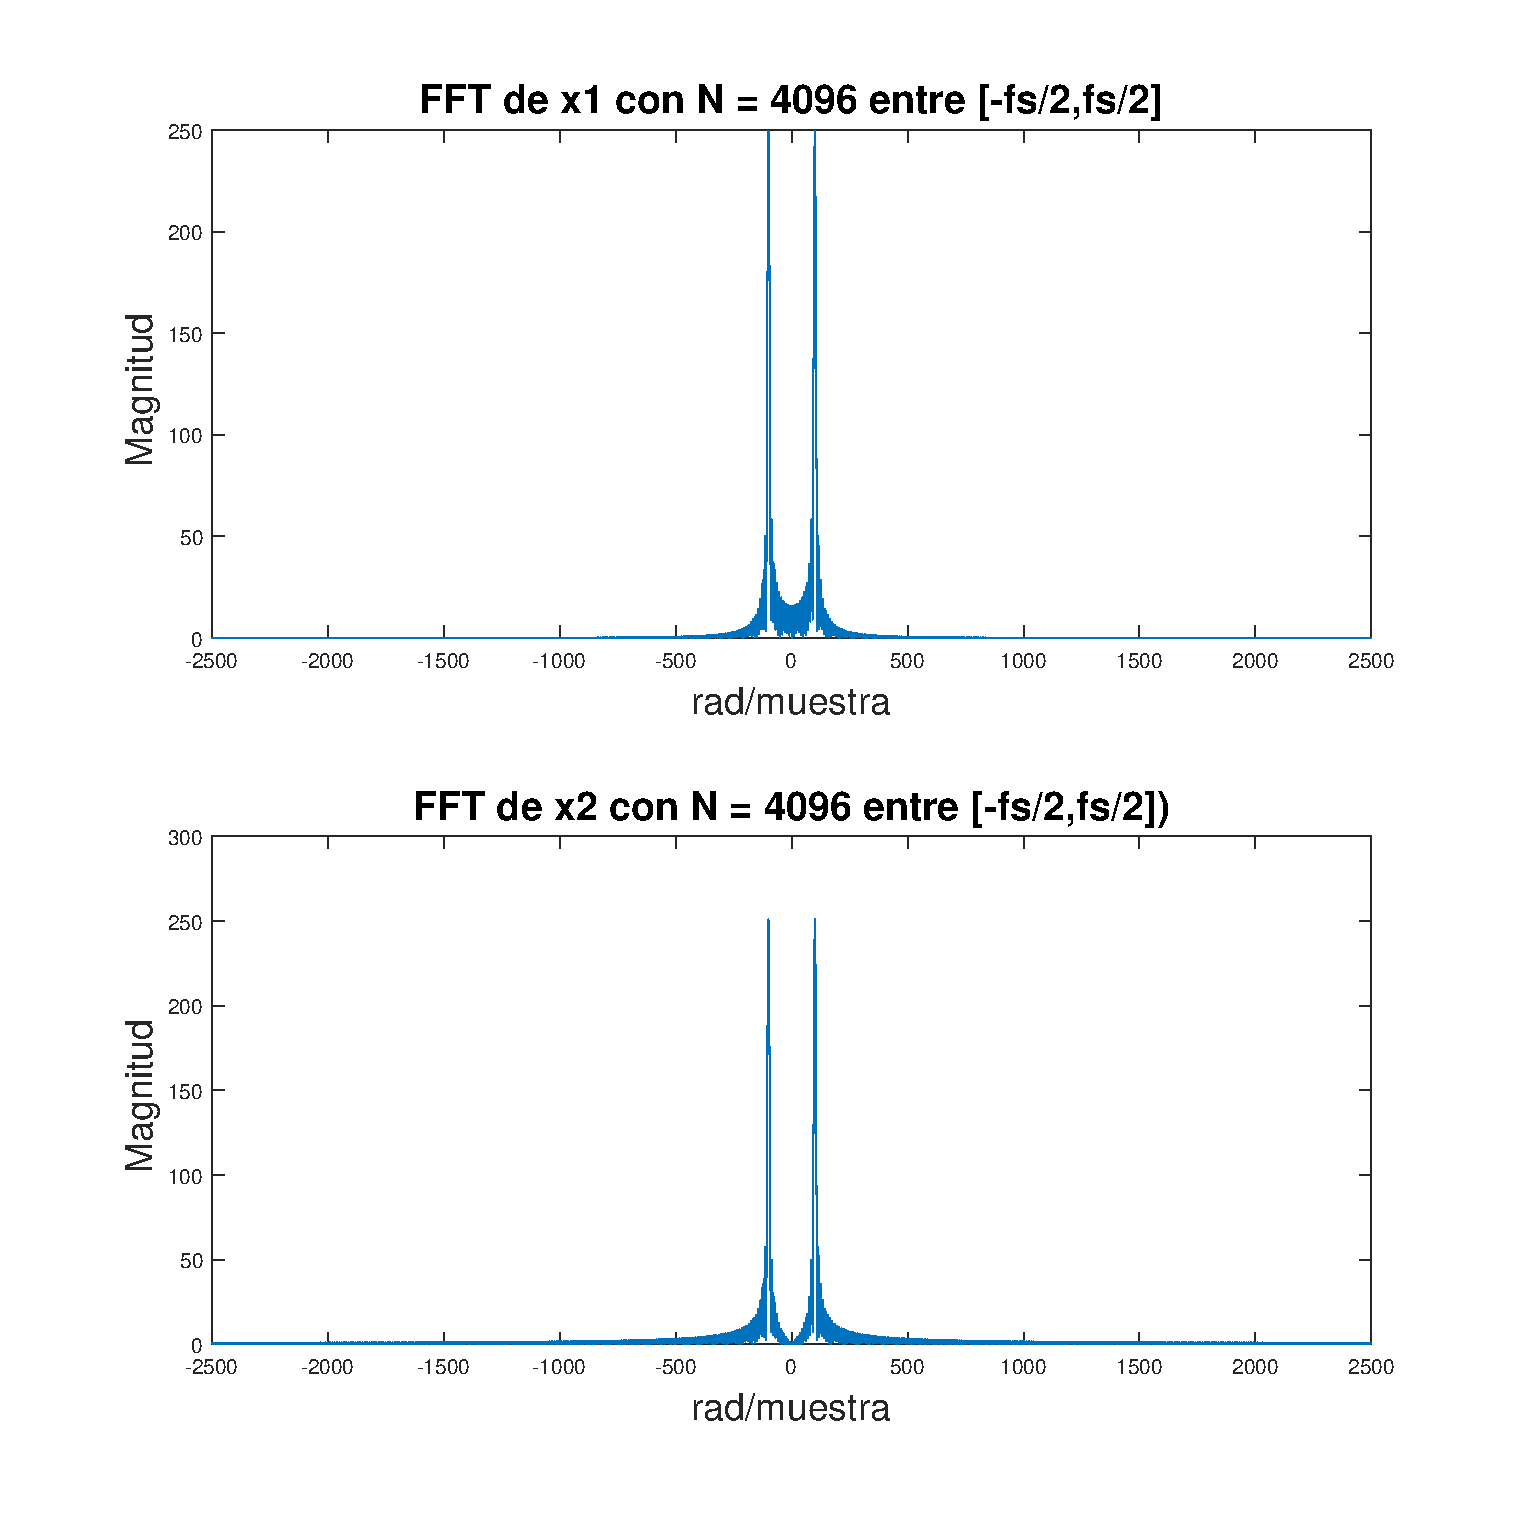
\includegraphics[scale = 0.6]{Figuras/p1_2-fs-medios.eps}
        \caption{Magnitud de la fft para las señales $x_1$ y $x_2$ entre   $[-\frac{fs}{2},\frac{fs}{2}]$ con N = 4096}
        \label{fs-medios}
    \end{figure}
    
        \begin{figure}[H]
        \centering
        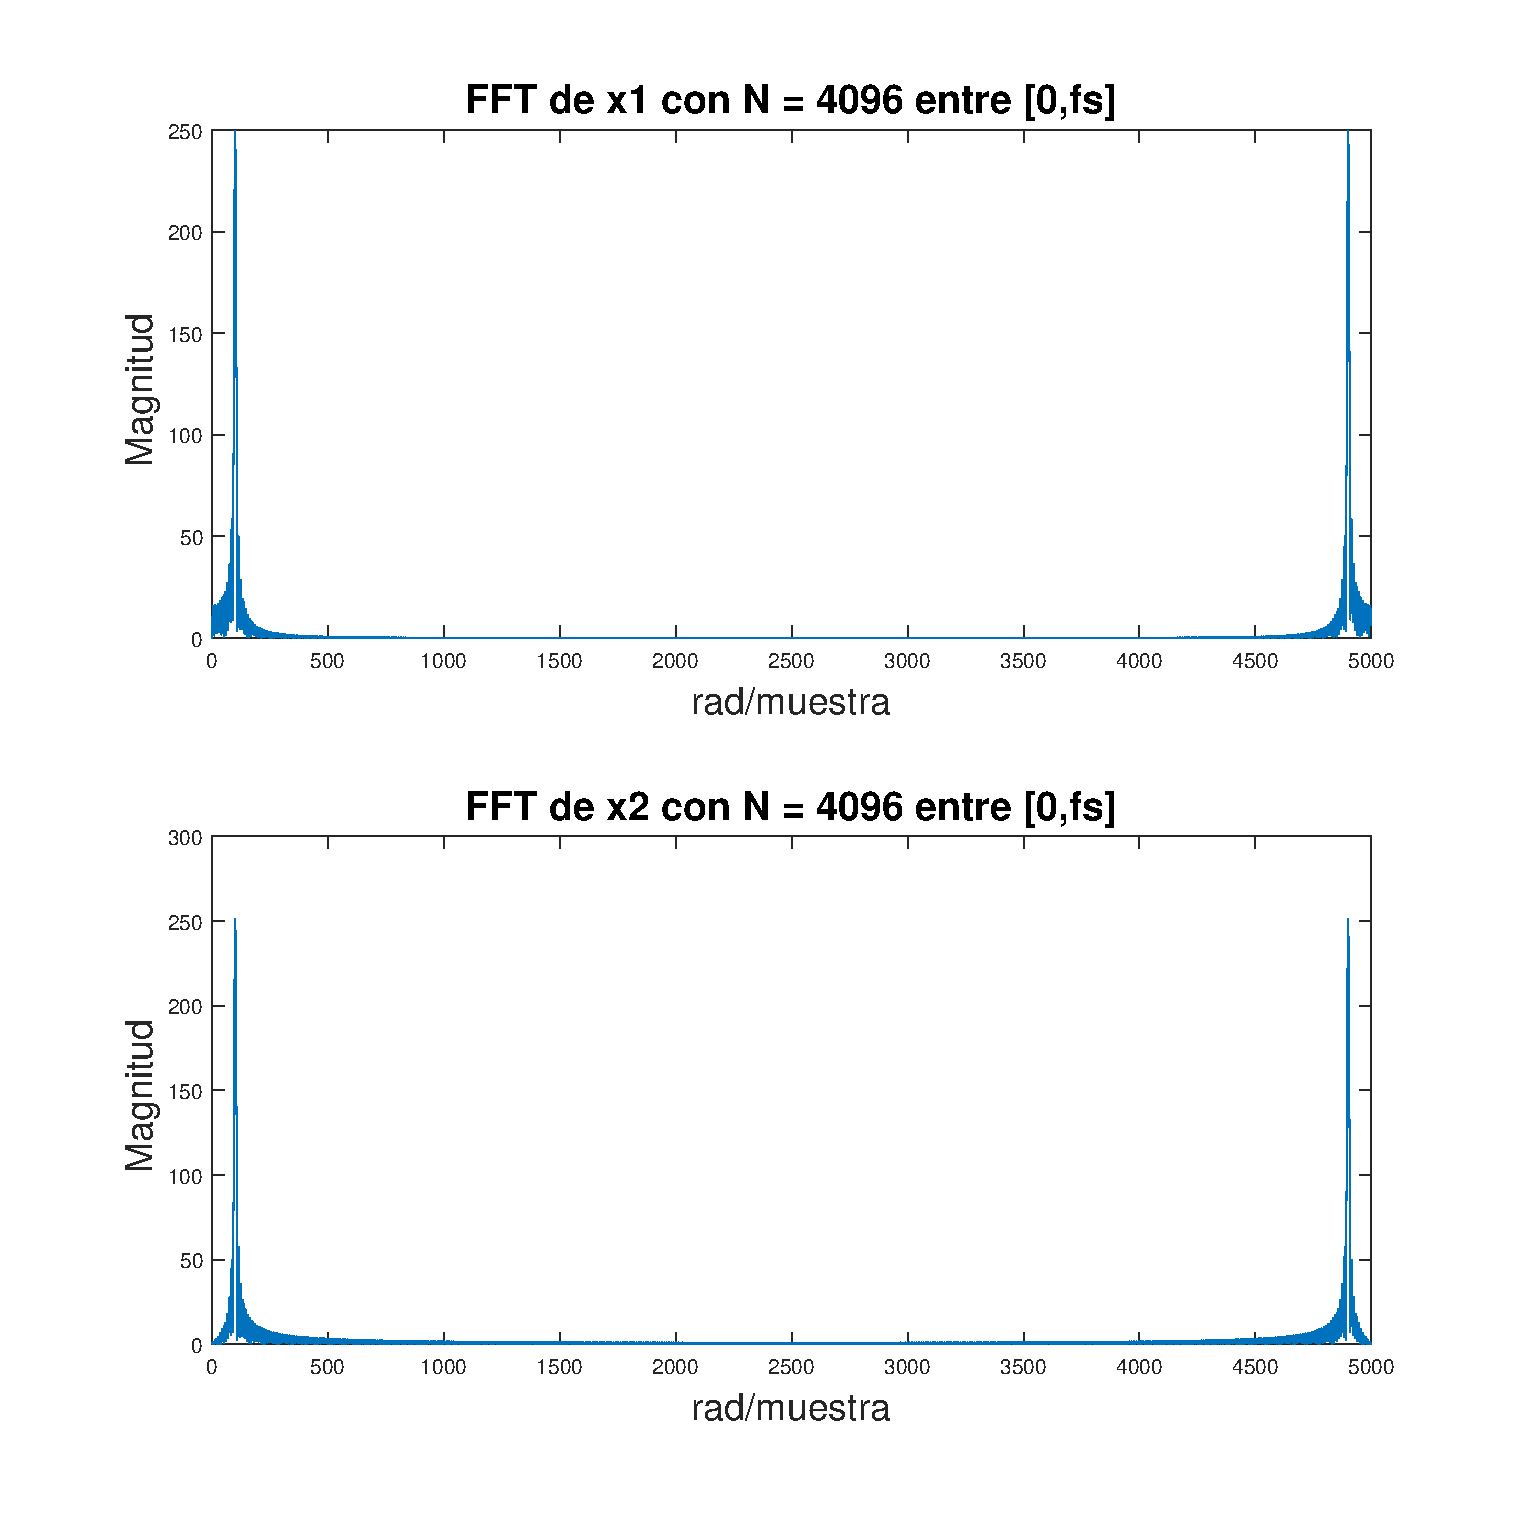
\includegraphics[scale = 0.6]{Figuras/p1_2-cero-fs-medio.eps}
        \caption{Magnitud de la fft para las señales $x_1$ y $x_2$ entre   $[0,\frac{fs}{2}]$ con N = 4096}
        \label{cero-fs-medio}
    \end{figure}


En las gráficas de ambas figuras se puede observar que el espectro tiene una amplitud de 250, lo que tiene sentido ya que este valor corresponde a la suma de todas las muestras y en este caso eran señales de 500 muestras, esto además de el factor de $\frac{1}{2}$ asociado a la transformada de Fourier de señales sinusoidales hace que los resultados obtenidos coincidan con los esperados.

\item Se obtiene la DFT de cada una de las señales anteriores, $x_1 $ y $x_2$,  para  valores de $N = 256$, $N = 500$ y $N = 2048$, luego se obtienen gráficos de magnitud $v/s$ Frecuencia además de la parte real y parte imaginaria $v/s$ frecuencia. Las gráficas obtenidas para $x_1$ se muestran en la figura \ref{x1} mientras que las correspondientes a la señal $x_2$ se encuentran en la figura \ref{x2}

\begin{figure}[H]
    \centering
    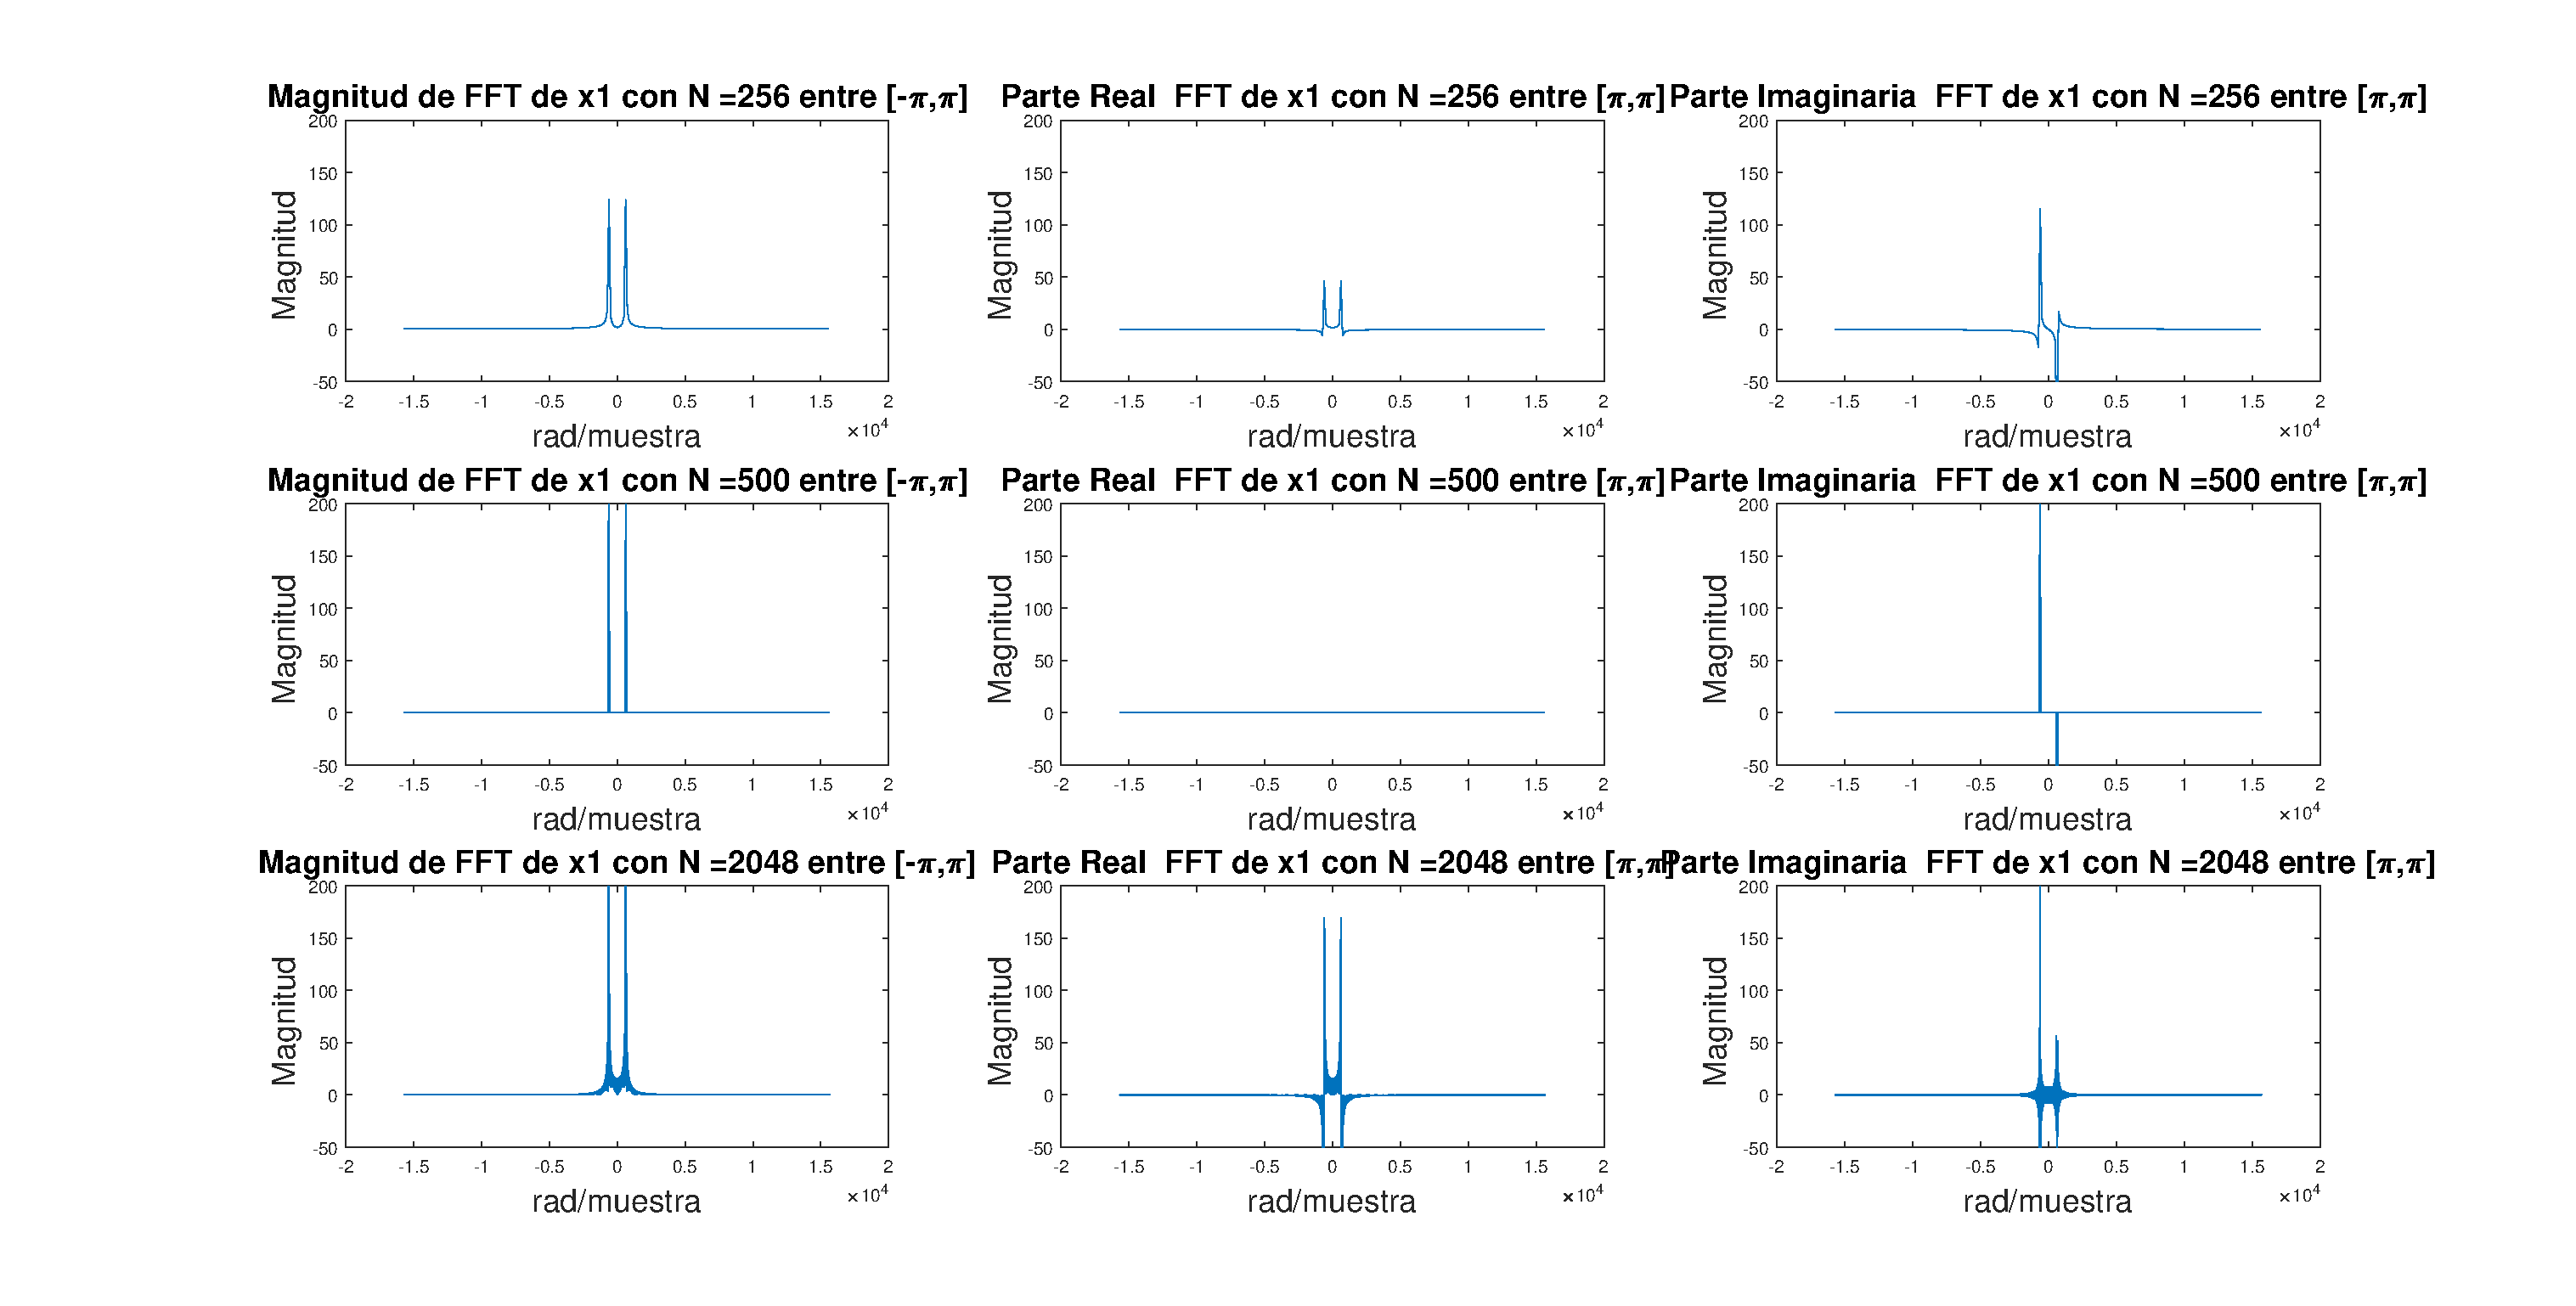
\includegraphics[scale = 0.3]{Figuras/p1_3-x1.eps}
    \caption{Magnitud y partes real e imaginaria de la señal $x_1 = sin(\omega t)$ para $N = 256,500,2048$}
    \label{x1}
\end{figure}

\begin{figure}[H]
    \centering
    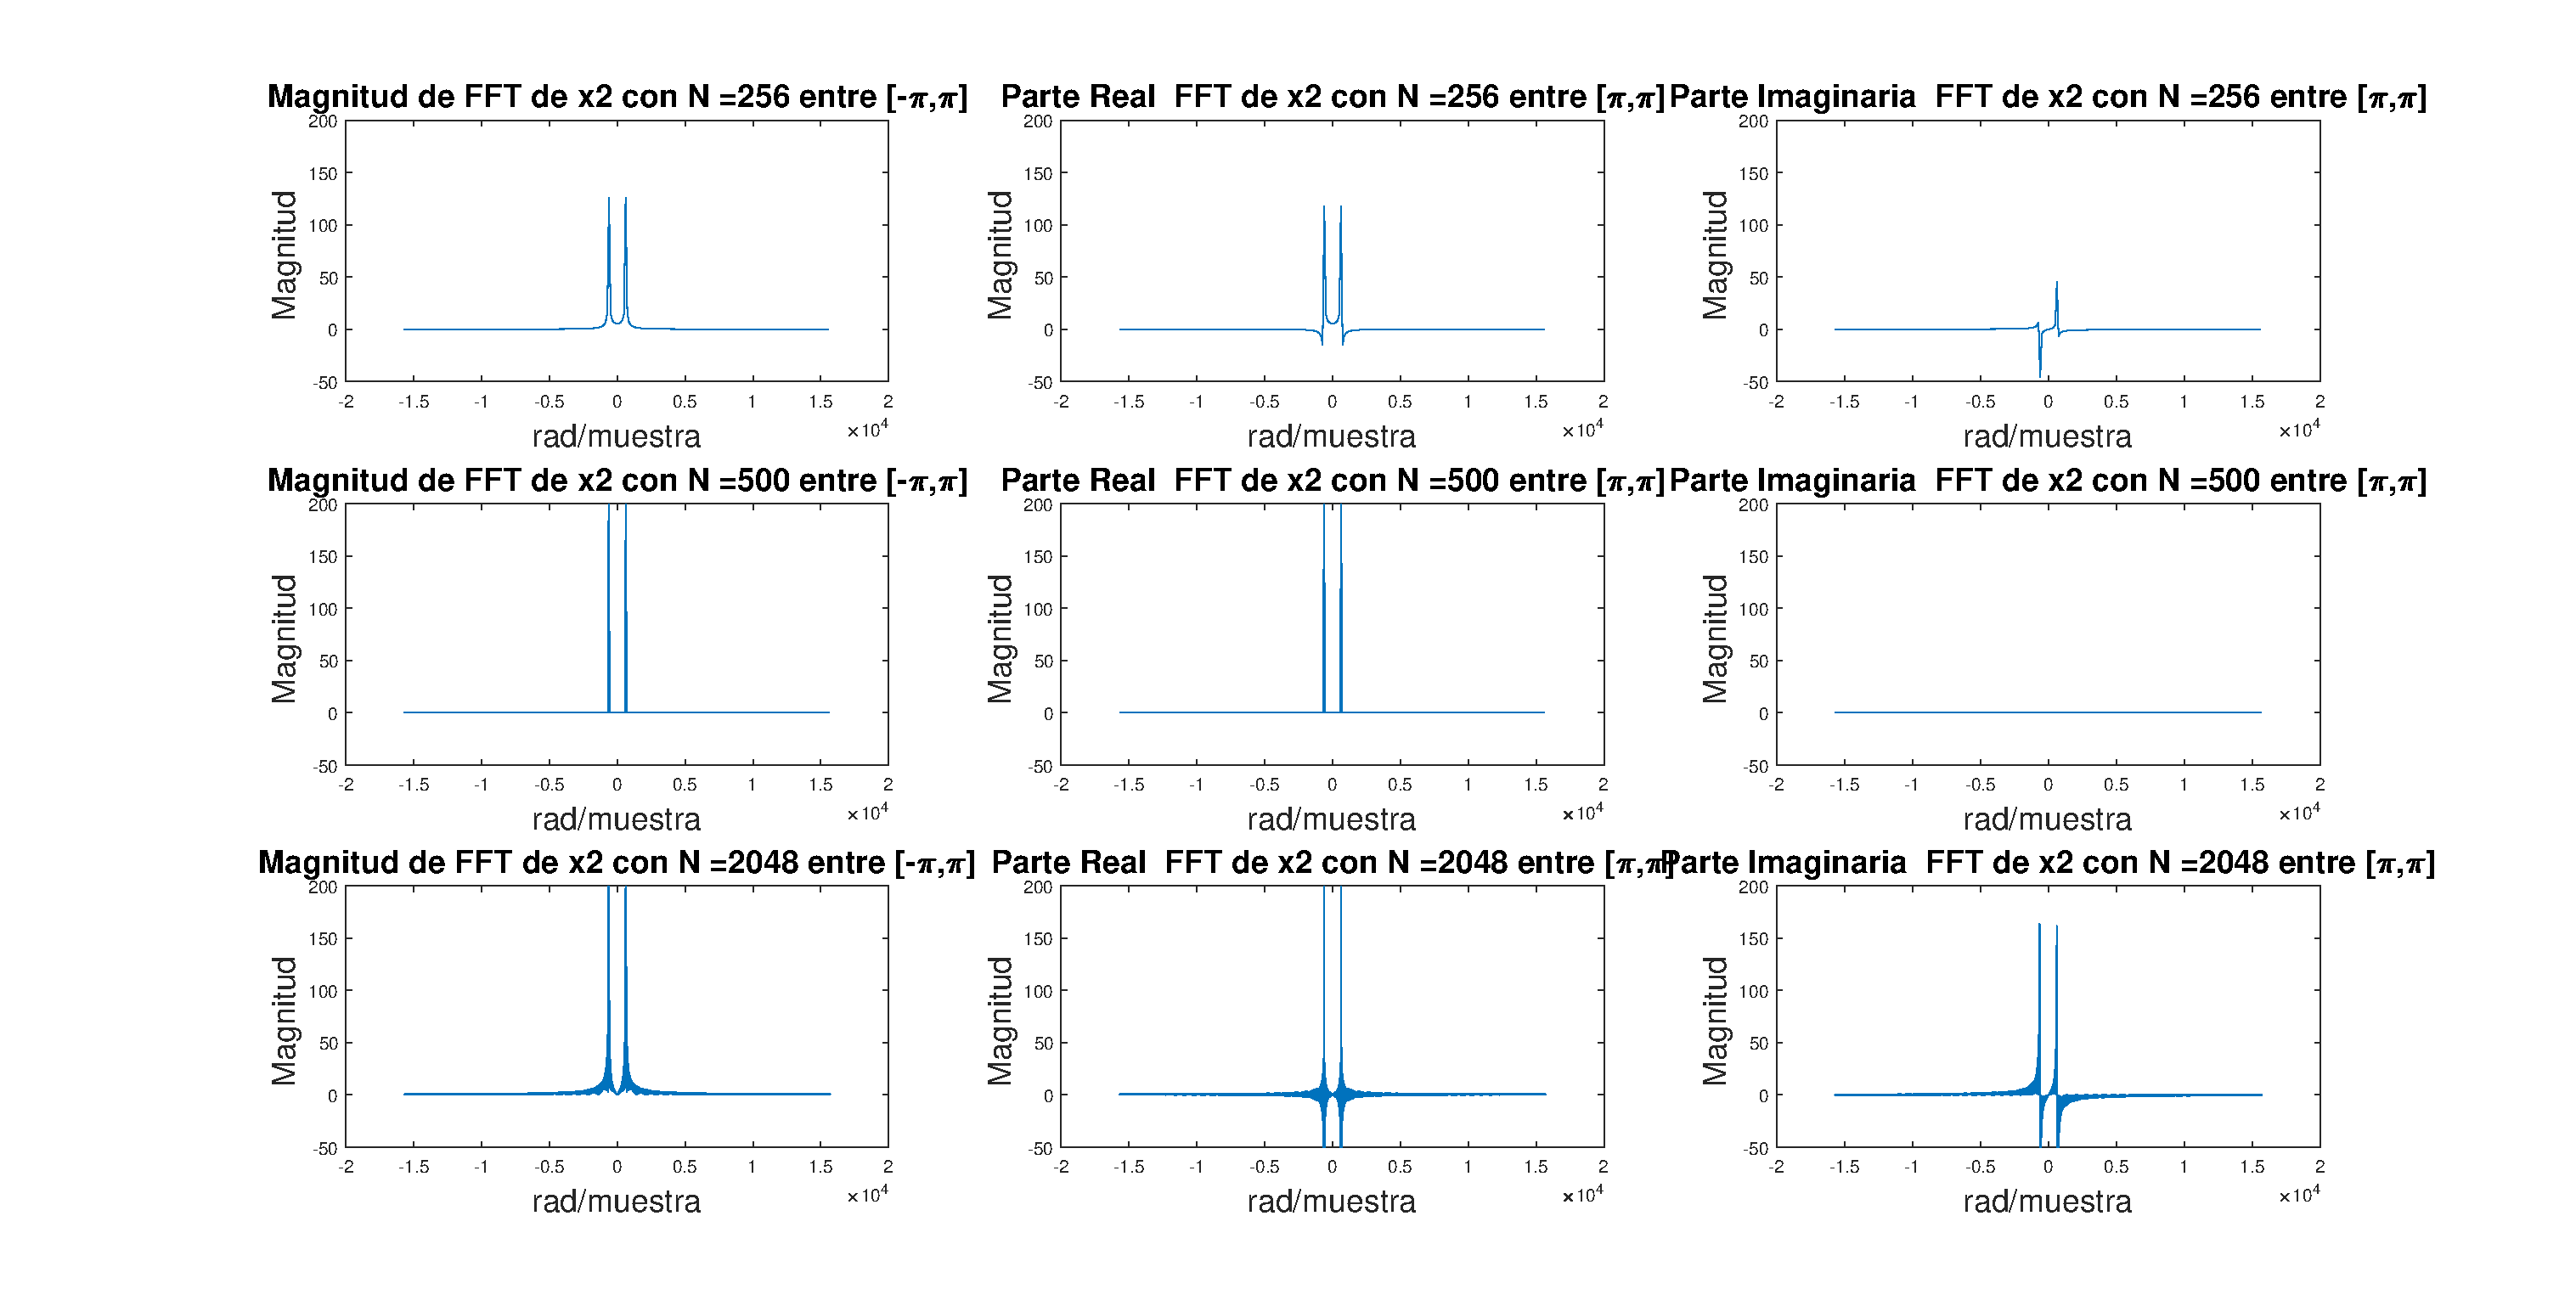
\includegraphics[scale = 0.3]{Figuras/p1_3-x2.eps}
    \caption{Magnitud y partes real e imaginaria de la señal $x_2 = cos(\omega t)$ para $N = 256,500,2048$}
    \label{x2}
\end{figure}

De las gráficas anteriores se puede concluir que el valor de N más apropiado es de 500, ya que los resultados obtenidos son los espectros más prolijos y cercanos a lo que se espera teóricamente de la transformada de ambas señales en caso de ser infinitas, esto se debe a que el $N=500$ permite que los bines de frecuencia  coincidan con las señales $sinc $ asociadas a las ventanas usadas en la transformación. 

En caso que se busque un resultado cercano para señales finitas el valor que proporciona mejores resultados es de $N = 2048$, en las graficas obtenidas con este N se pueden apreciar los lóbulos laterales que se generan por las ventanas asociadas a la transformación.





\end{enumerate}

\newpage
\section{Estimación de frecuencia en presencia de ruido}
Se genera una señal de 2 tonos puros de 100 y 500 Hz con amplitudes $0,5$ y $1,5$ respectivamente. Se le agrega a esta señal ruido blanco de distribución normal de media 0 y varianza 2, muestreando la señal resultante durante 100 ms a $f_s = 2000~Hz$ para cumplir con el criterio de Nyquist.

En la figura \ref{fig:p2_1t} se muestra la representación temporal de la señal con ruido. A partir del gráfico no es posible reconocer que la señal limpia corresponde a la superposición de 2 tonos puros ni las frecuencias de estos.

\begin{figure}[H]
    \centering
    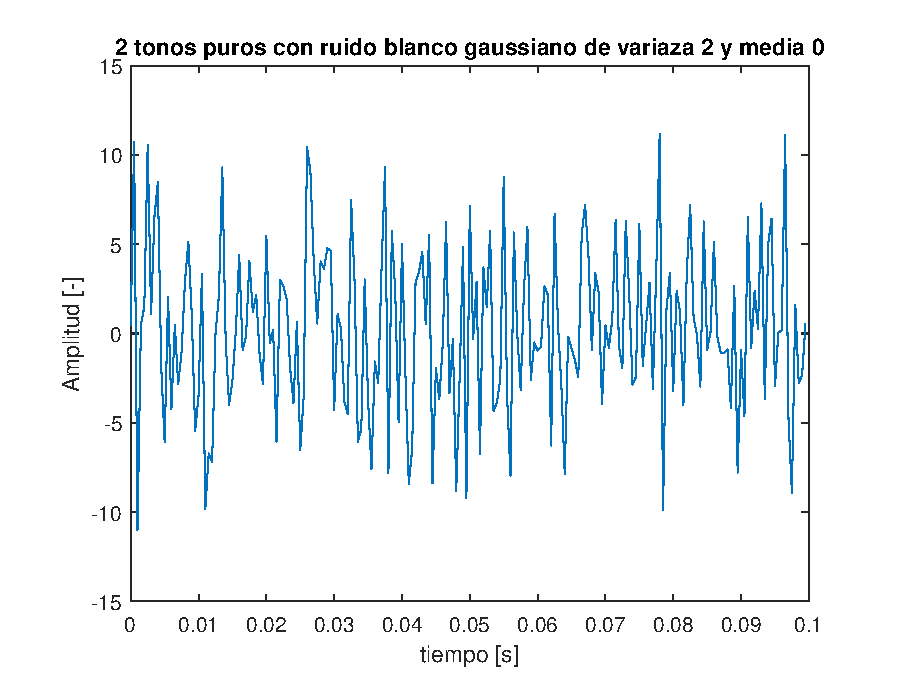
\includegraphics[width = .8\linewidth]{Figuras/1.eps}
    \caption{Representación temporal de señal de 2 tonos puros con ruido}
    \label{fig:p2_1t}
\end{figure}

Luego se grafica la magnitud del espectro de las señales con y sin ruido usando el comando $fft()$ de MATLAB. Dichos gráficos se muestran en la figura \ref{fig:p2_2mag} 

\begin{figure}[H]
    \centering
    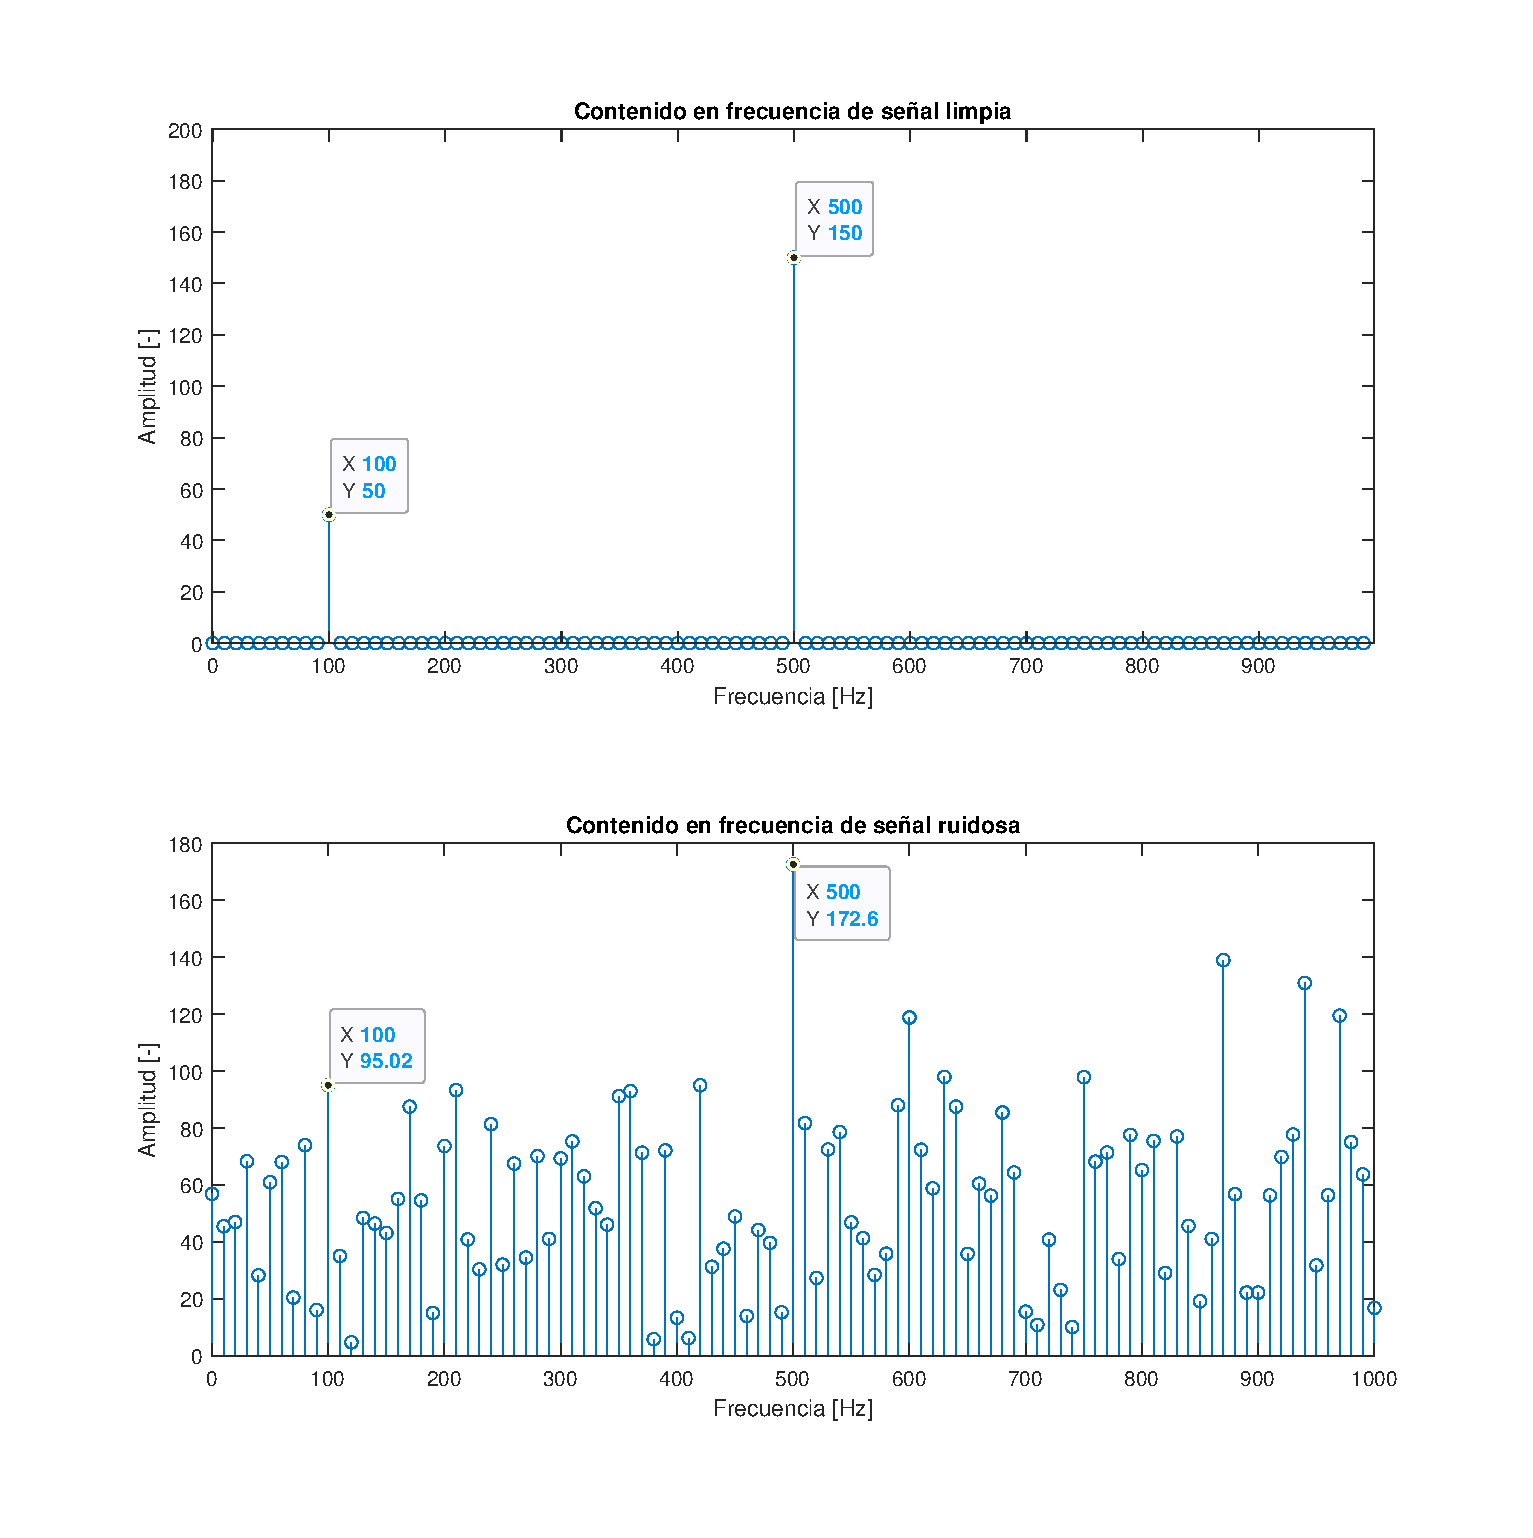
\includegraphics[width = .8\linewidth]{Figuras/2.eps}
    \caption{Magnitud del espectro de señal de 2 tonos puros sin y con ruido.}
    \label{fig:p2_2mag}
\end{figure}

Con respecto a la figura \ref{fig:p2_2mag} se aprecia que la amplitud de los tonos puros no es la misma en ambos casos. Lo anterior se debe a que el ruido agregado también tiene contenido en frecuencia en las frecuencias de los tonos puros.

Posteriormente se grafica la magnitud en dB del espectro en frecuencia de las señales con y sin ruido, normalizando la amplitud máxima a 0 dB. Dicho gráfico se muestra en la figura \ref{fig:p2_3mag}. En el caso de la señal limpia se observa que la diferencia de amplitud entre la componenente más elevada y el piso de ruido es de -300 dB aproximadamente. En el caso de la señal ruidosa es de aproximadamente -10 dB. 

\begin{figure}[H]
    \centering
    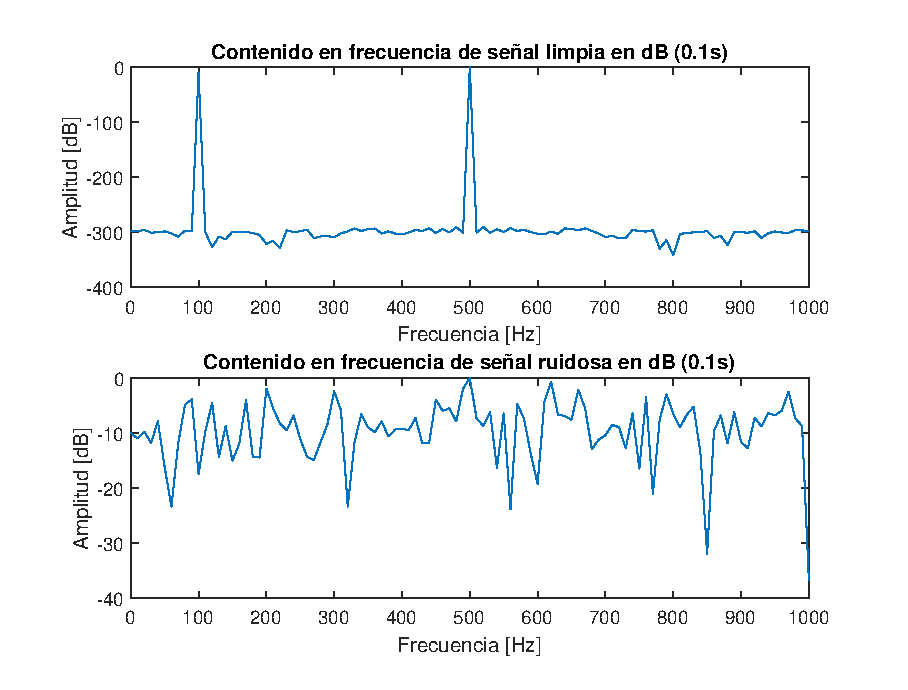
\includegraphics[width = .8\linewidth]{Figuras/3.eps}
    \caption{Magnitud en decibeles del espectro de señal de 2 tonos puros sin y con ruido, de duración 1 ms.}
    \label{fig:p2_3mag}
\end{figure}

%cCOMENTARIOS AMPLITUD

Finalmente se cambia la duración de la señal a 1s y se vuelve a graficar la magnitud normalizada en dB del espectro en frecuencia de las señales con y sin ruido. Dicho gráfico se muestra en la figura \ref{fig:p2_4mag}. Las diferencias entre el espectro encontrado con una ventana de 1 s y 0.1 s se debe a que la ventana de mayor largo en frecuencia es más angosta, lo que se traduce en un menor \textit{leakage}.

\begin{figure}[H]
    \centering
    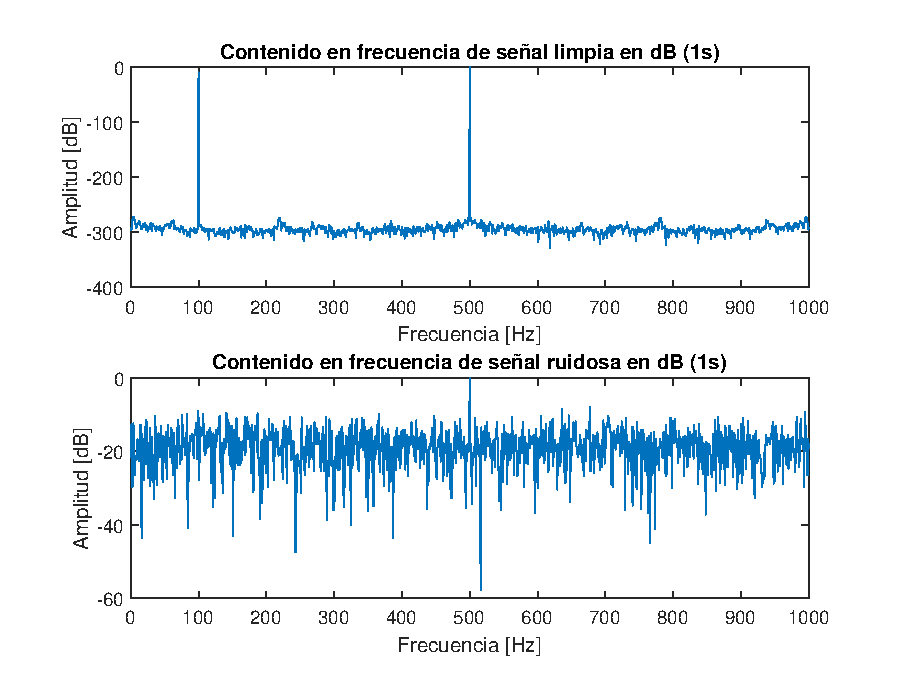
\includegraphics[width = .8\linewidth]{Figuras/4.eps}
    \caption{Magnitud en decibeles del espectro de señal de 2 tonos puros sin y con ruido, de duración 1 s.}
    \label{fig:p2_4mag}
\end{figure}

\newpage
\section{Filtrado de señales en el dominio de la frecuencia}
Se pide hacer un filtrado en frecuencia del archivo \texttt{nspeech.mat}, el cual presenta un tono molesto.

En primer lugar se obtiene la DFT de dicha señal y se grafica su magnitud en frecuencia, encontrando un peak en los 1685 Hz, localizando así el tono molesto. El gráfico obtenido se muestra en la figura \ref{fig:p3_1cf}.

\begin{figure}[H]
    \centering
    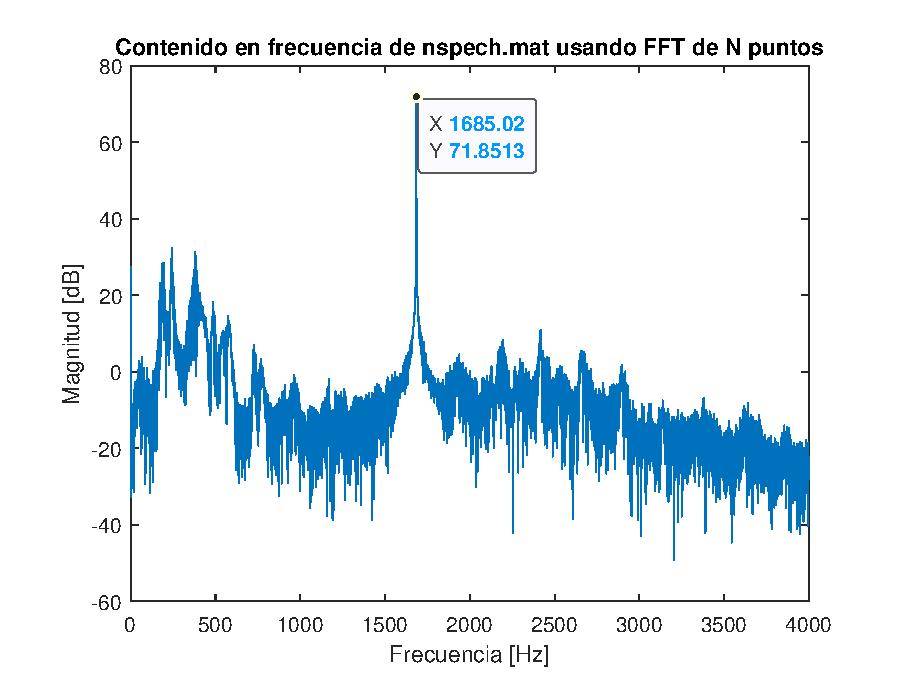
\includegraphics[width = .8\linewidth]{Figuras/p3_1cf.eps}
    \caption{Contenido en frecuencia (magnitud) de señal \texttt{nspeech.mat}.}
    \label{fig:p3_1cf}
\end{figure}

Posteriormente se diseña un filtro de 2 ceros conjugados, de respuesta en frecuencia:
$$ H(\omega) = 1-2\cos{(\theta)e^{-j\omega}+e^{-2j\omega}}$$
Donde se ubican los ceros en el ángulo correspondiente a la frecuencia normalizada del tono molesto, es decir 
$$ \theta = 2\pi \dfrac{f_0}{f_s} =2\pi \dfrac{1685}{8000} = 1.322~ \dfrac{\text{rad}}{\text{muestra}}$$
Con el objetivo de penalizar dicha frecuencia. La magnitud de la respuesta en frecuencia del filtro diseñado se muestra en la figura \ref{fig:p3_2rfH}. Se aprecia la penalización correspondiente en la frecuencia del tono molesto. 

\begin{figure}[H]
    \centering
    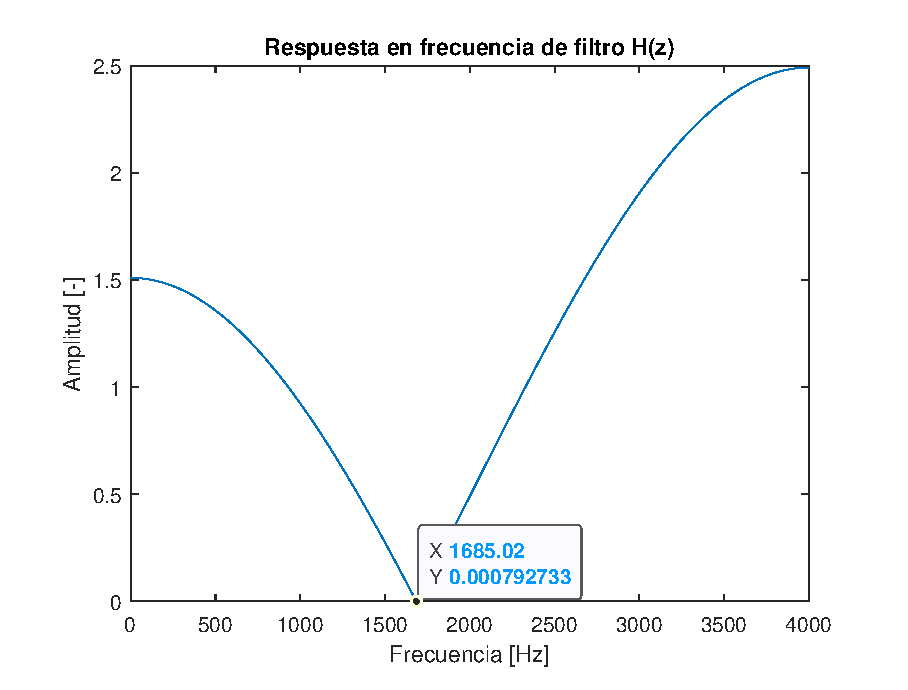
\includegraphics[width = .8\linewidth]{Figuras/p3_2rfH.eps}
    \caption{Respuesta en frecuencia (magnitud) de filtro de 2 ceros complejos conjugados diseñado.}
    \label{fig:p3_2rfH}
\end{figure}

Ya con el filtro diseñado, se realiza el filtrado en frecuencia haciendo un producto punto a punto de las respuestas en frecuencia del contenido en frecuencia de la señal \texttt{nspeech.mat} y la respuesta en frecuencia de $H$, teniendo cuidado con que la discretización en frecuencia de la expresión de $H(\omega)$ corresponda a la frecuencia de los bines de la DFT de la señal original.

La magnitud del contenido en frecuencia de la señal filtrada se muestra en la figura \ref{fig:p3_3cffilt}. En comparación con la figura \ref{fig:p3_1cf} se aprecia una gran atenuación, más no eliminación del tono molesto. Lo anterior se le atribuye a temas numéricos.

\begin{figure}[H]
    \centering
    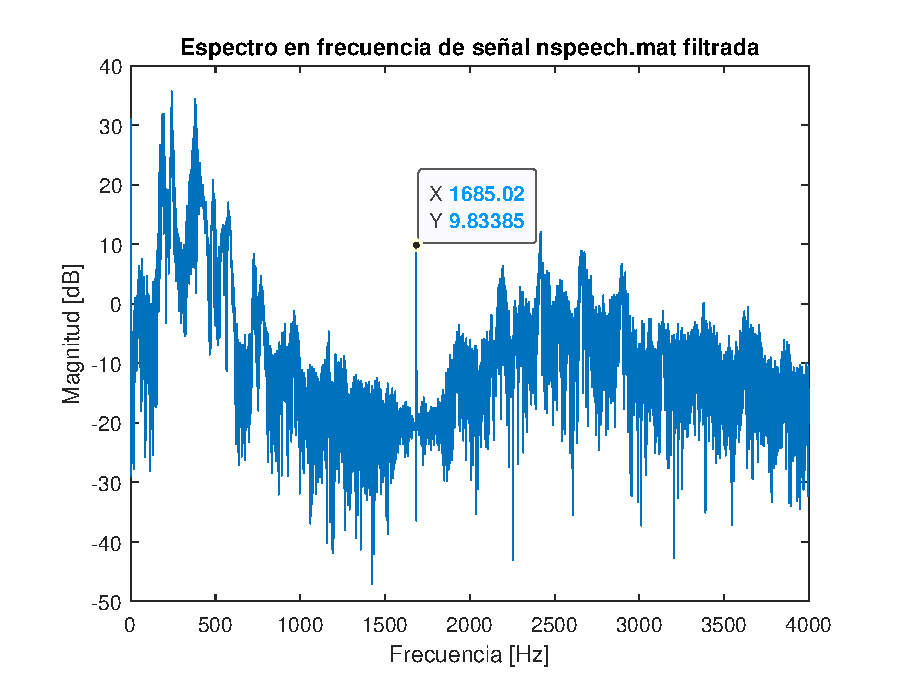
\includegraphics[width = .8\linewidth]{Figuras/p3_3cffilt.eps}
    \caption{Contenido en frecuencia (magnitud) de señal \texttt{nspeech.mat} filtrada.}
    \label{fig:p3_3cffilt}
\end{figure}

Finalmente se aplica la DFT inversa a la señal filtrada en el dominio de la frecuencia para obtener su representación en el dominio del tiempo. Los gráficos de la señal pre y post filtrado se muestran en la figura \ref{fig:p3_4tiempo}. Visualmente aprecian buenos resultados producto al filtrado. Con respecto al número de puntos para recuperar la señal completa, corresponde al número de puntos de la señal \texttt{nspeech.mat}.

\begin{figure}[H]
    \centering
    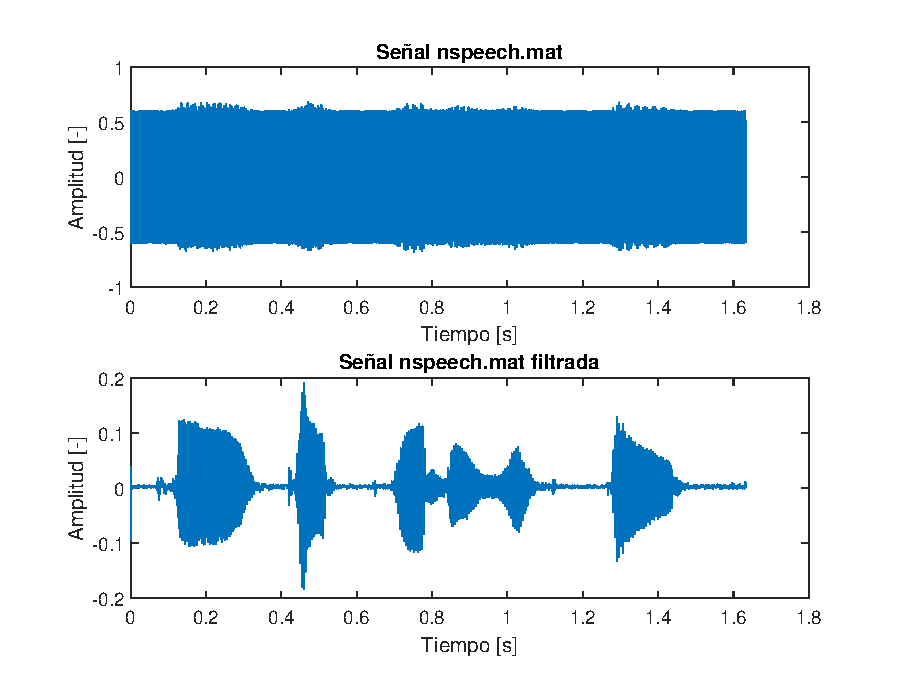
\includegraphics[width = .8\linewidth]{Figuras/p3_4tiempo.eps}
    \caption{Representación de señal pre y post filtrado en el dominio temporal.}
    \label{fig:p3_4tiempo}
\end{figure}

Con respecto a la percepción auditiva, se aprecia una gran disminución del tono molesto, sin embargo, sigue sonando levemente. Se adjuntan archivos de audio \texttt{nspeech\_filtered.wav} y \texttt{nspeech\_unfiltered.wav} a la entrega.

\newpage
\section{Cálculo directo de la DFT}
Para efectuar el calculo directo de la DFT haciendo uso de la herramienta MATLAB se implementa la función \texttt{X= DFTsum(x)} para obtener la DFT de N puntos, siendo \texttt{x} el parámetro corresponde a una señal de entrada \textit{x(n)} la cual desarrolla la ecuación \ref{DFT} en base a \textit{ciclos-for} calculando a la vez los exponenciales directamente. Esta código de implementación de la función se presenta a continuación

\begin{lstlisting}[language = octave]
function X = DFTsum(x)
    N = length(x);
    X = zeros(1,N);
    for k = 0:N-1
        coef = exp(-1j*2*pi*k/N);
        for n = 0:N-1
            X(1,k+1) = X(1,k+1) + x(n+1)*coef^n;
          
        end
        
    end
    
end
\end{lstlisting}


\begin{equation}
    X_N(k) = X^{(N)}(k) = \sum_{n = 0}^{N-1} x(n)e^{-j2\pi k n /N}
    \label{DFT}
\end{equation}

\begin{enumerate}
    \item Para probar la función implementada se generaron las siguientes señales 
    
    $$ x_1(n) = \delta (n)$$
    $$ x_2(n) = 1$$
    $$ x_3(n) =e^{-j2 \pi n /N}$$
    $$ x_4(n) = cos(2\pi n /N)$$
    
    
    Se grafica la salida de la función en el rango $[-\pi, \pi]$ para cada señal considerando 8 muestras para cada una, se  grafica además, en el mismo rango de valores el resultado que entrega MATLAB al aplicar el comando \texttt{fft} a las señales generadas. Las gráficas mencionadas se muestran en la figura \ref{DFTsum}
    
    \begin{figure}[H]
        \centering
        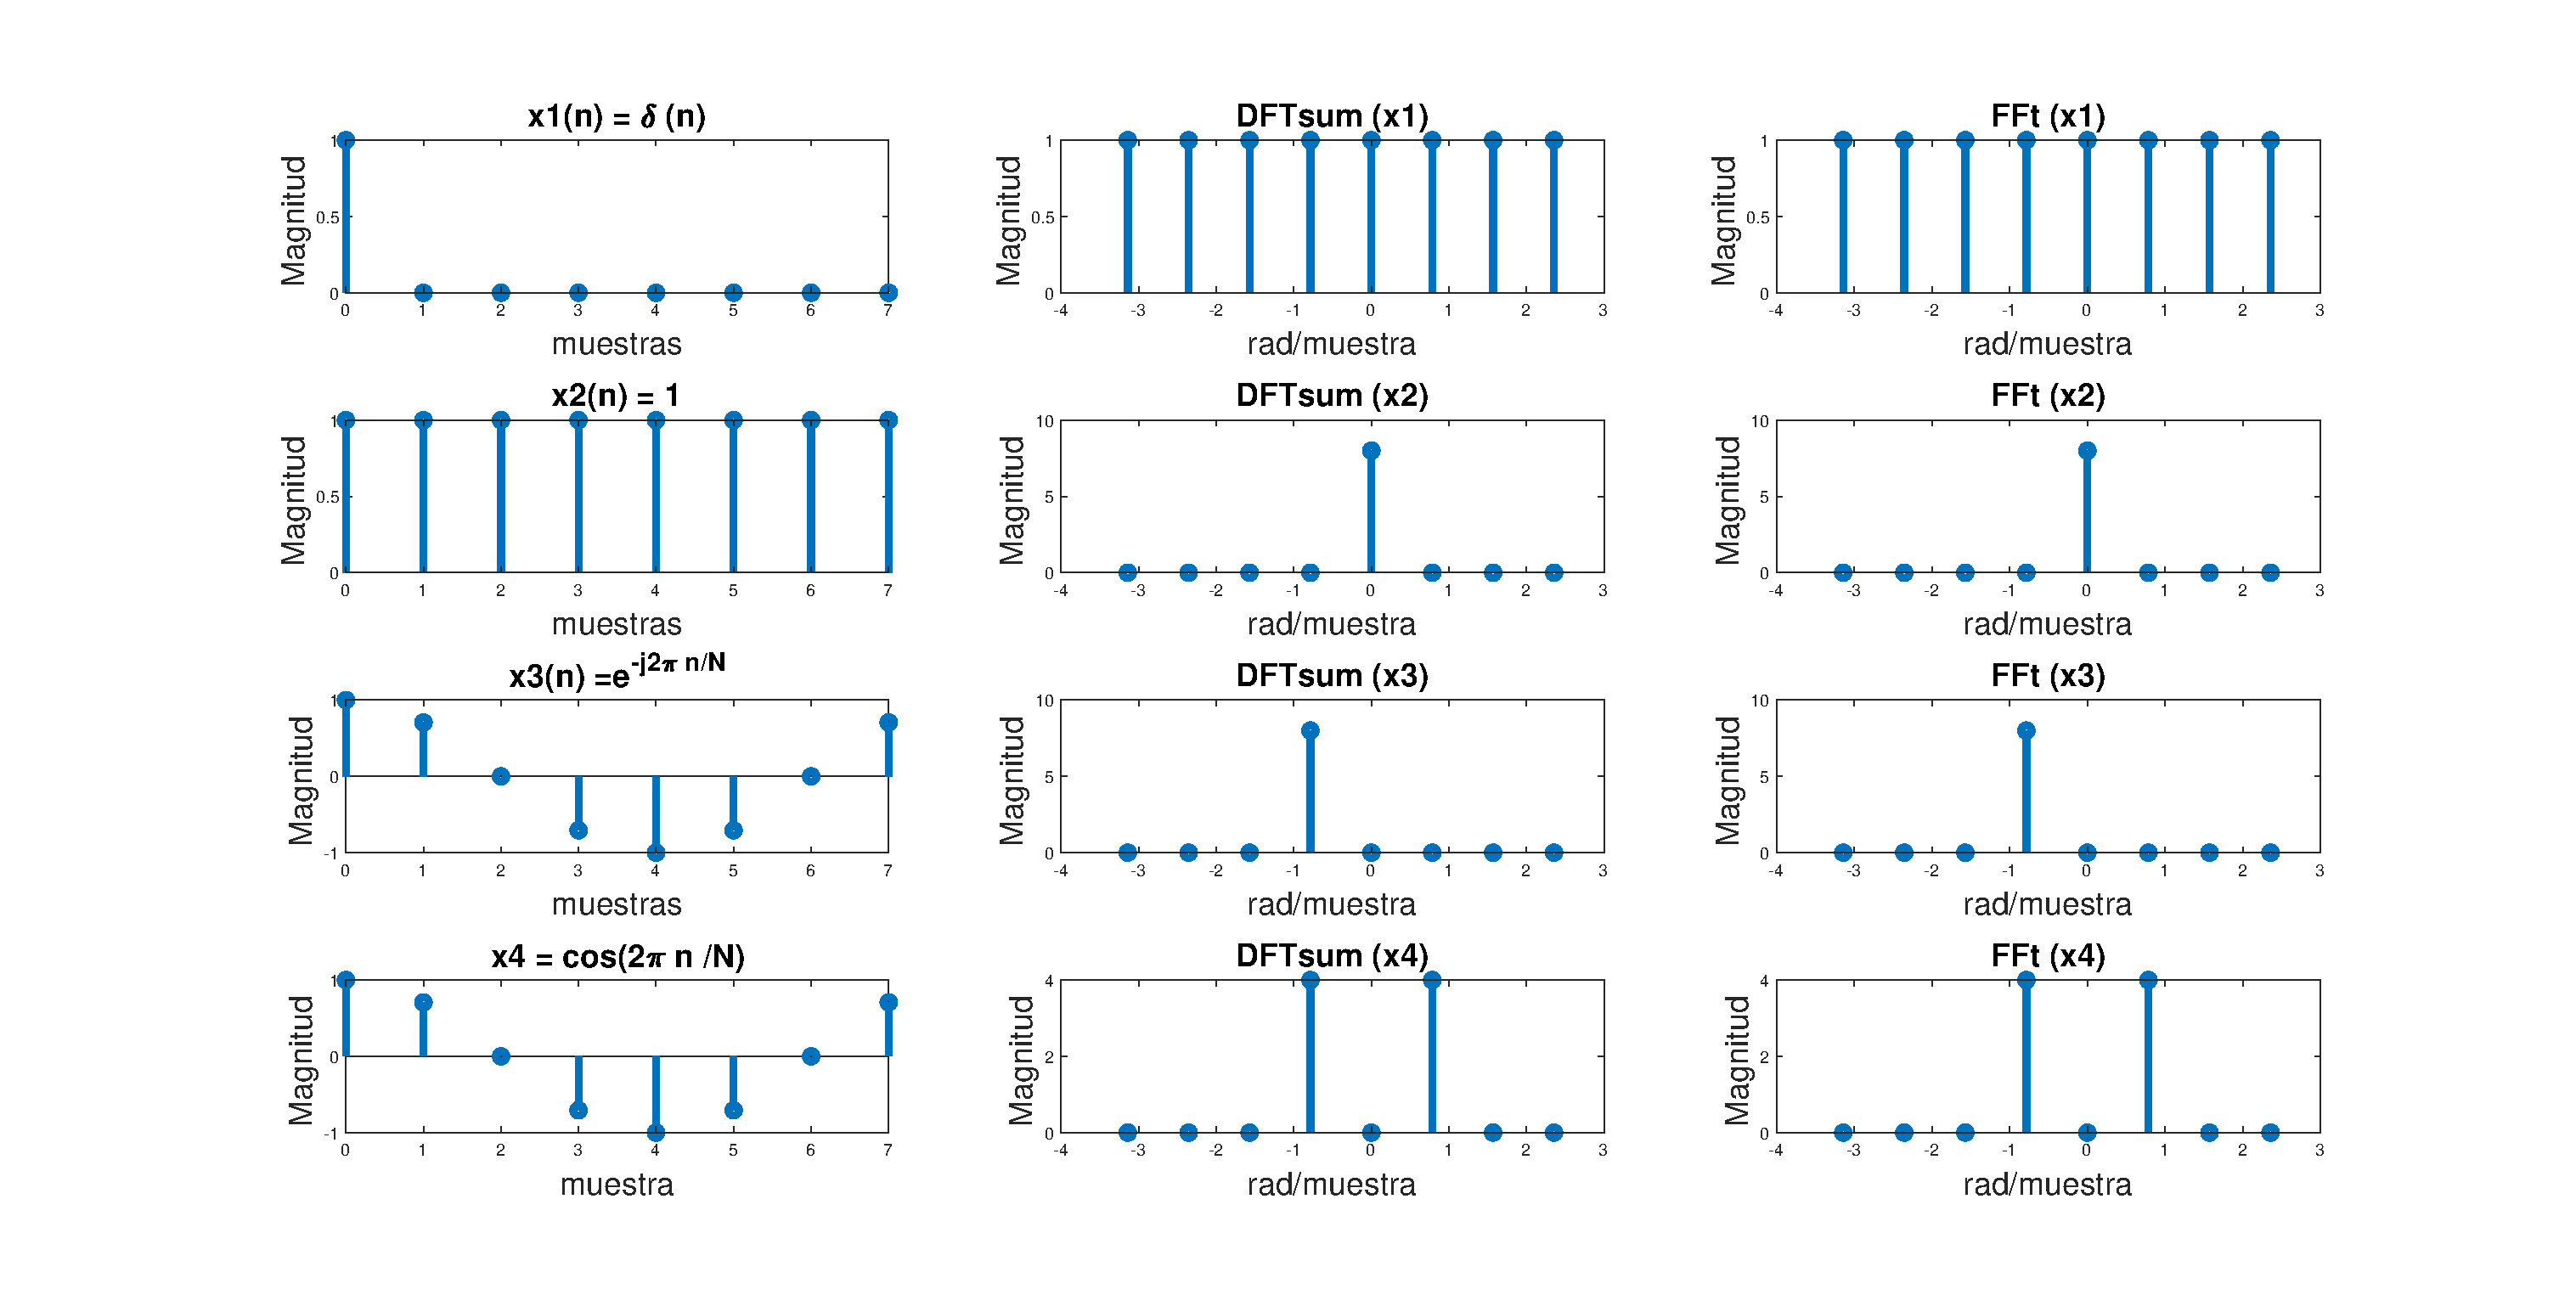
\includegraphics[scale = 0.3]{Figuras/p4_1-DFTsum.eps}
        \caption{Señales $x_1$, $x_2$, $x_3$ y $x_4$ generadas junto a sus respectivas DFT obtenida con la función implementada y FFT obtenida con comandos en MATLAB}
        \label{DFTsum}
    \end{figure}


Se puede apreciar cómo el resultado que se obtiene mediante el comando \texttt{fft} de MATLAB es idéntico al que se obtiene al utilizar la función \texttt{DFTsum} siendo consistente con lo que se espera de su funcionamiento según la teoría. En el caso particular de la señal $x_3$ que corresponde a una señal compleja se presenta  gráfica solo de la parte real asociada a su espectro en frecuencia por lo que el resultado es similar al de la señal $x_4$ pero con un solo impulso (\textit{recordar $2cos(\phi) = e^{j\phi} + e^{j\phi}$}).


Usando el comando de MATLAB \texttt{immse} se obtuvo la siguiente tabla resumen entre los valores numéricos obternidos usando la función \texttt{DFTsum} y el resultado entregado por el comando \texttt{fft} de MATLAB


 \begin{table}[H]
        \centering
        \begin{tabular}{|c|c|}
        \hline
         Señal    & MSE $DFT~~ v/s~~ fft$  \\
         \hline
         $x_1(n) = \delta (n)$   & $0$ \\
         \hline
          $x_2(n) = 1$   &   $1.2195\cdot 10^{-30}$ \\
         \hline
            $ x_3(n) =e^{-j2 \pi n /N}$ &   $7.1631\cdot 10^{-31} $\\
         \hline
        
         $ x_4(n) = cos(2\pi n /N)$  &    $3.1880\cdot 10{-31}  $\\
         \hline


        \end{tabular}
        \caption{Cuadro resumen para el error cuadrático medio entre el resultado de la función \texttt{DFTsum} y el resultado entregado por el comando \texttt{fft} de MATLAB para cada señal de prueba.}
        \label{MSE}
    \end{table}
    
    %4.2
    \item
    
    
    %4.3
    \item Se considera la señal $x_1(t) = cos(wt)$ con frecuencia de 100 Hz, muestreada a 5kHz durante 1000 ms. 
    
    Se grafica el error en la magnitud del espectro obtenido con la función \texttt{DFTsum} y \texttt{fft}. Dicho gráfico se muestra en la figura \ref{fig:p4_3err}, donde se observa un máximo error del orden de $10^{-9}$, por lo que se asume despreciable. El error cuadrático medio obtenido es de $5.4744 \cdot 10^{-22}$.
    
    \begin{figure}[H]
        \centering
        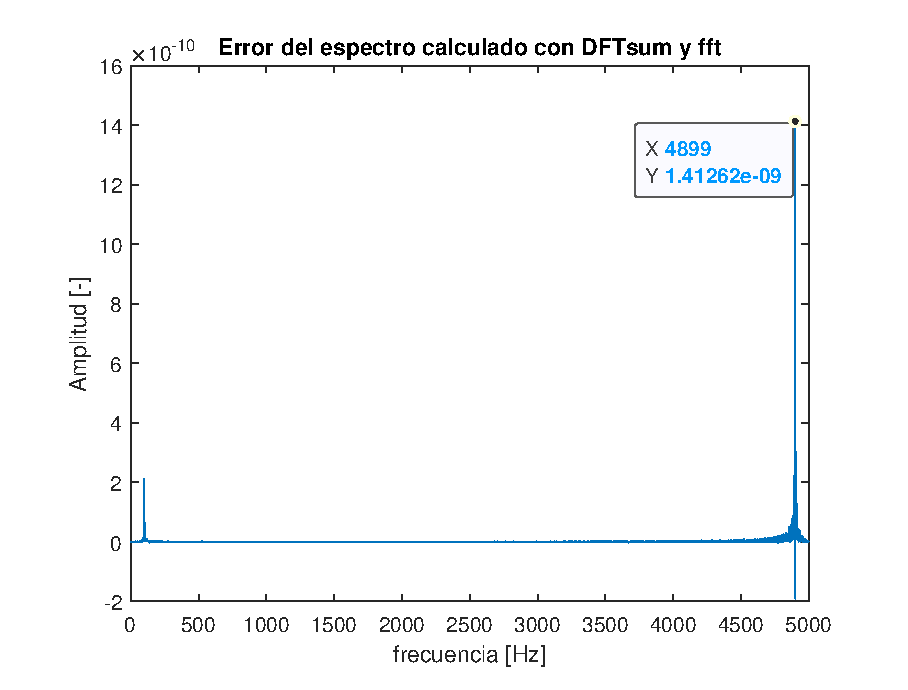
\includegraphics[width = 0.8\linewidth]{Figuras/p4_3err.eps}
        \caption{Error de magnitud del espectro utilizando \texttt{DFTsum} con respecto a \texttt{fft} en MATLAB.}
        \label{fig:p4_3err}
    \end{figure}
     
     

    

    
\end{enumerate}



\newpage
\section{Cálculo matricial de la DFT}
  \begin{enumerate}
      \item En esta sección se busca poder obtener la DFT de gracias a un  como un producto entre una matriz y un vector, de modo que $X = Ax$, donde $X$ y $x$ son vectores columna de $N\times1$ y $A$ es una matriz cuadrada de $N\times N$. Este producto es equivalente a $$X_k = \sum_{n=1}^{N}A_{k n}X_n$$
      donde $A_{k n}$ es el elemento $(k, n)$ de la matriz dado por 
      $$A_{k n} =e^{-j 2 \pi (k-1)(n-1)/N}$$
      
      Para poder implementar esta forma en primera instancia se debe implementa la función \texttt{genAmatrix(N)}, para lo que se utilizó el siguiente código en base a \textit{ciclos-for}
      
      \begin{lstlisting}[language = octave]
function A = genAmatrix(N)
    A = zeros(N,N);
    
    for k =1:N
        for  n = 1:N
            A(k,n) = exp(-1j*2*pi*(k-1)*(n-1)/N);
        end
        
    end
    
end

      \end{lstlisting}

  
  
  Para evaluar la función generadora de la matriz A se compara sus resultados con los que se obtienen al generar la misma matriz con elcomando \textit{dftmtx} de MATLAB para los valores N = 2,4,8,16 y  32 . Se  el error cuadrático medio entre ambos métodos, obteniendo datos que se presentan en la siguiente tabla
  
  
  
 \begin{table}[H]
        \centering
        \begin{tabular}{|c|c|}
        \hline
         N    & MSE $genAmatrix(N) ~ v/s~~ dftmtx$  \\
         \hline
         2  & $ 3.749\cdot 10^{-33}$ \\
         \hline
        4  &   $4.5930\cdot 10^{-32}$ \\
         \hline
        8  & $7.9370\cdot 10^{-31} $\\
         \hline
        
         16&    $7.7116\cdot 10^{-30} $\\
         \hline
         
         32&    $ 3.1181\cdot 10^{-29} $\\
         \hline



        \end{tabular}
        \caption{Cuadro resumen para el error cuadrático medio entre el resultado de la función \texttt{genAmatrix(N)} y el resultado entregado por el comando \texttt{dftmtx} de MATLAB para N = 2,4,8,16 y 32.}
        \label{MSE_Amatrix}
    \end{table}
    
    
    Todos los errores obtenidos son despreciables para fines prácticos debido al orden de magnitud que poseen en comparación a los valores que se utilizan en los cálculos de interés.
    
    Para poder efectuar finalmente el cálculo de la DFT mediante matrices se implementa la función \texttt{DFTmatrix(x)}, la que invoca a la función \texttt{genAmatrix(N)}. Para esto se utiliza el código que se presenta a continuación
    
    \begin{lstlisting}
function X = DFTmatrix(x)
    N = length(x);
    A = genAmatrix(N);
    X = sum(A'.*x');
end

    \end{lstlisting}
    
    %5.2
    \item Se pide graficar la parte imaginaria y la parte real de las matrices de DFT para $N = 8$ y $64$.
    
    Las matrices de la DFT de 8 puntos se muestran en la figura \ref{fig:p5_2n8}.
    
    Con respecto a la parte real se aprecia simetría con respecto a la diagonal principal (matriz simétrica). Sin consderar la primera fila y columna, se observa simetria con respecto a la columna y fila central.
    
    Con respecto a la parte imaginaria, se aprecia simetría con respecto a la diagonal principal (matriz simétrica). Sin consderar la primera fila y columna, se observa simetria con respecto también a la diagonal secundaria.
    
    \begin{figure} [H]
        \centering
        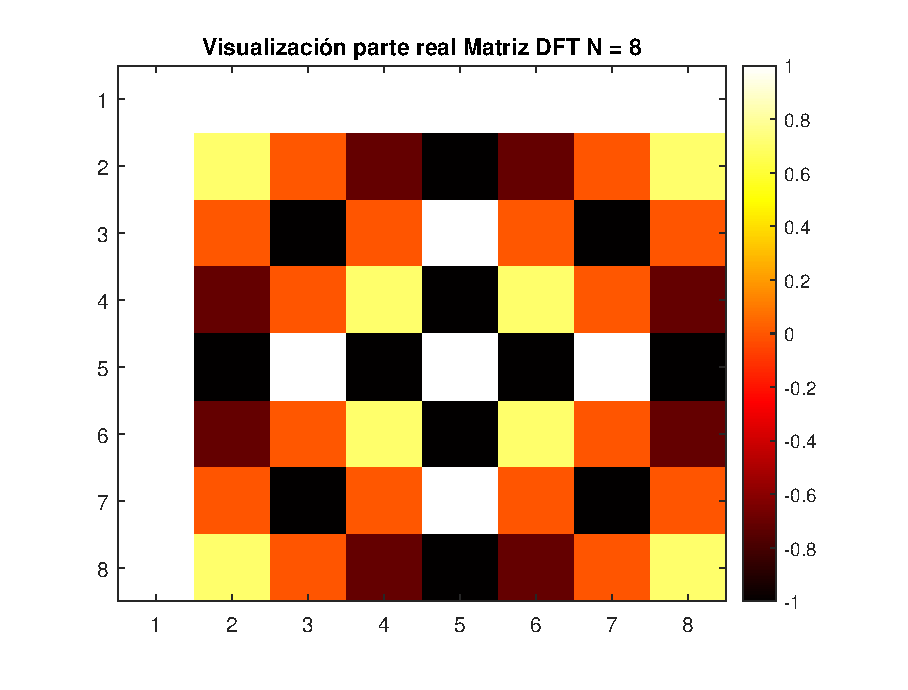
\includegraphics[width = .7\linewidth]{Figuras/P5_2_1.eps}
        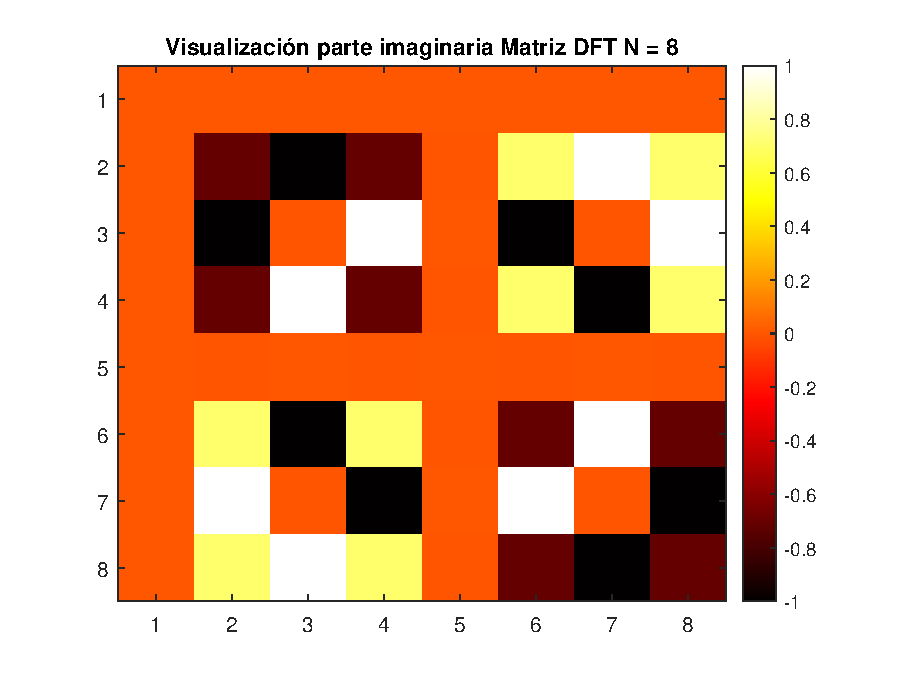
\includegraphics[width = .7\linewidth]{Figuras/P5_2_2.eps}
        \caption{Visualización parte real e imaginaria de matriz DFT de 8 puntos.}
        \label{fig:p5_2n8}
    \end{figure}
    
    Las matrices de la DFT de 64 puntos se muestran en la figura \ref{fig:p5_2n64}.
    
    No se aprecian diferencias en las simetrías apreciadas en la parte real e imaginaria con respecto a la matriz de 8 puntos.
    
    \begin{figure} [H]
        \centering
        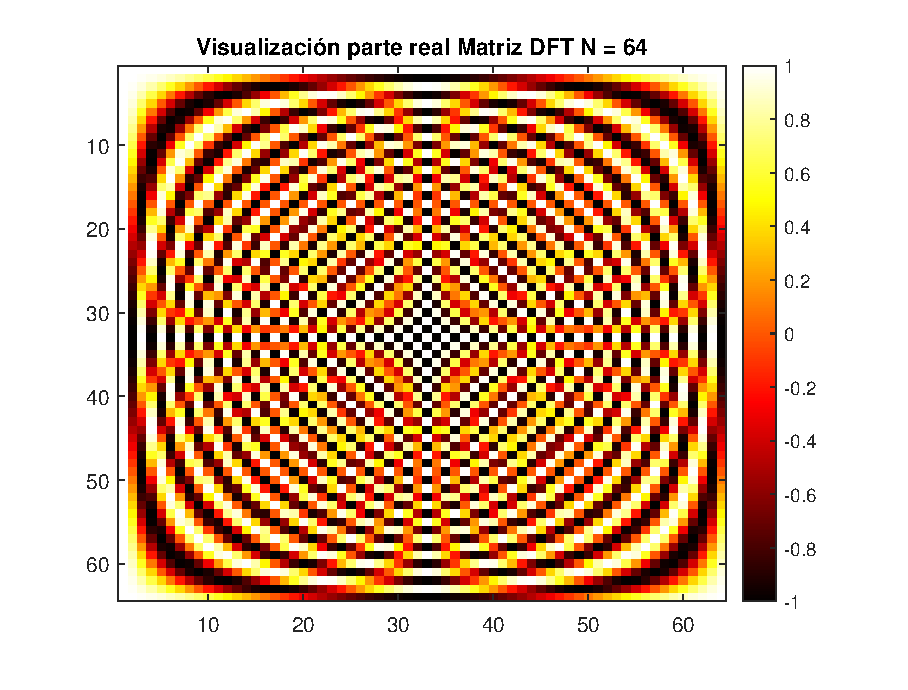
\includegraphics[width = .7\linewidth]{Figuras/P5_2_3.eps}
        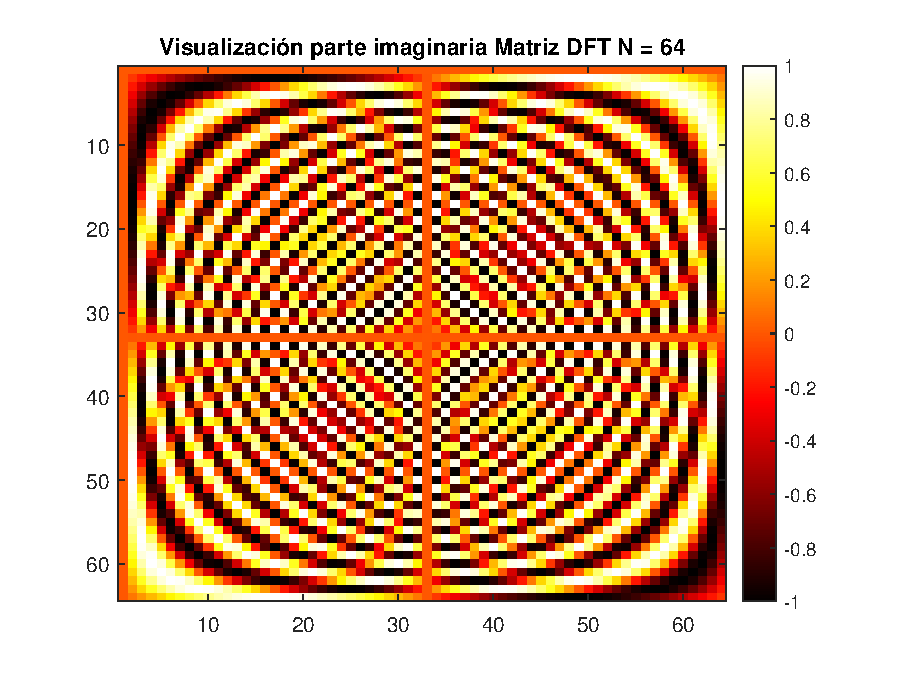
\includegraphics[width = .7\linewidth]{Figuras/P5_2_4.eps}
        \caption{Visualización parte real e imaginaria de matriz DFT de 64 puntos.}
        \label{fig:p5_2n64}
    \end{figure}
    
    
    %5.3
    \item Para probar la implementación de la función \texttt{DFTmatrix(x)}, se procede de la misma forma que al probar la implementación de la función \texttt{DFTsum(x)} del inciso anterior. Se usan las mismas señales $x1,x_2,x_3$ y $x_4$ también con 8 muestras para cada una de ellas. Se grafica la para cada señal el resultado entregado por la función implementada así como el resultado que se obtiene haciendo uso del comando \textit{fft} de MATLAB. Las gráficas mencionadas se muestran en la figura  \ref{DFTmatrix}
    
    
    \begin{figure}[H]
        \centering
        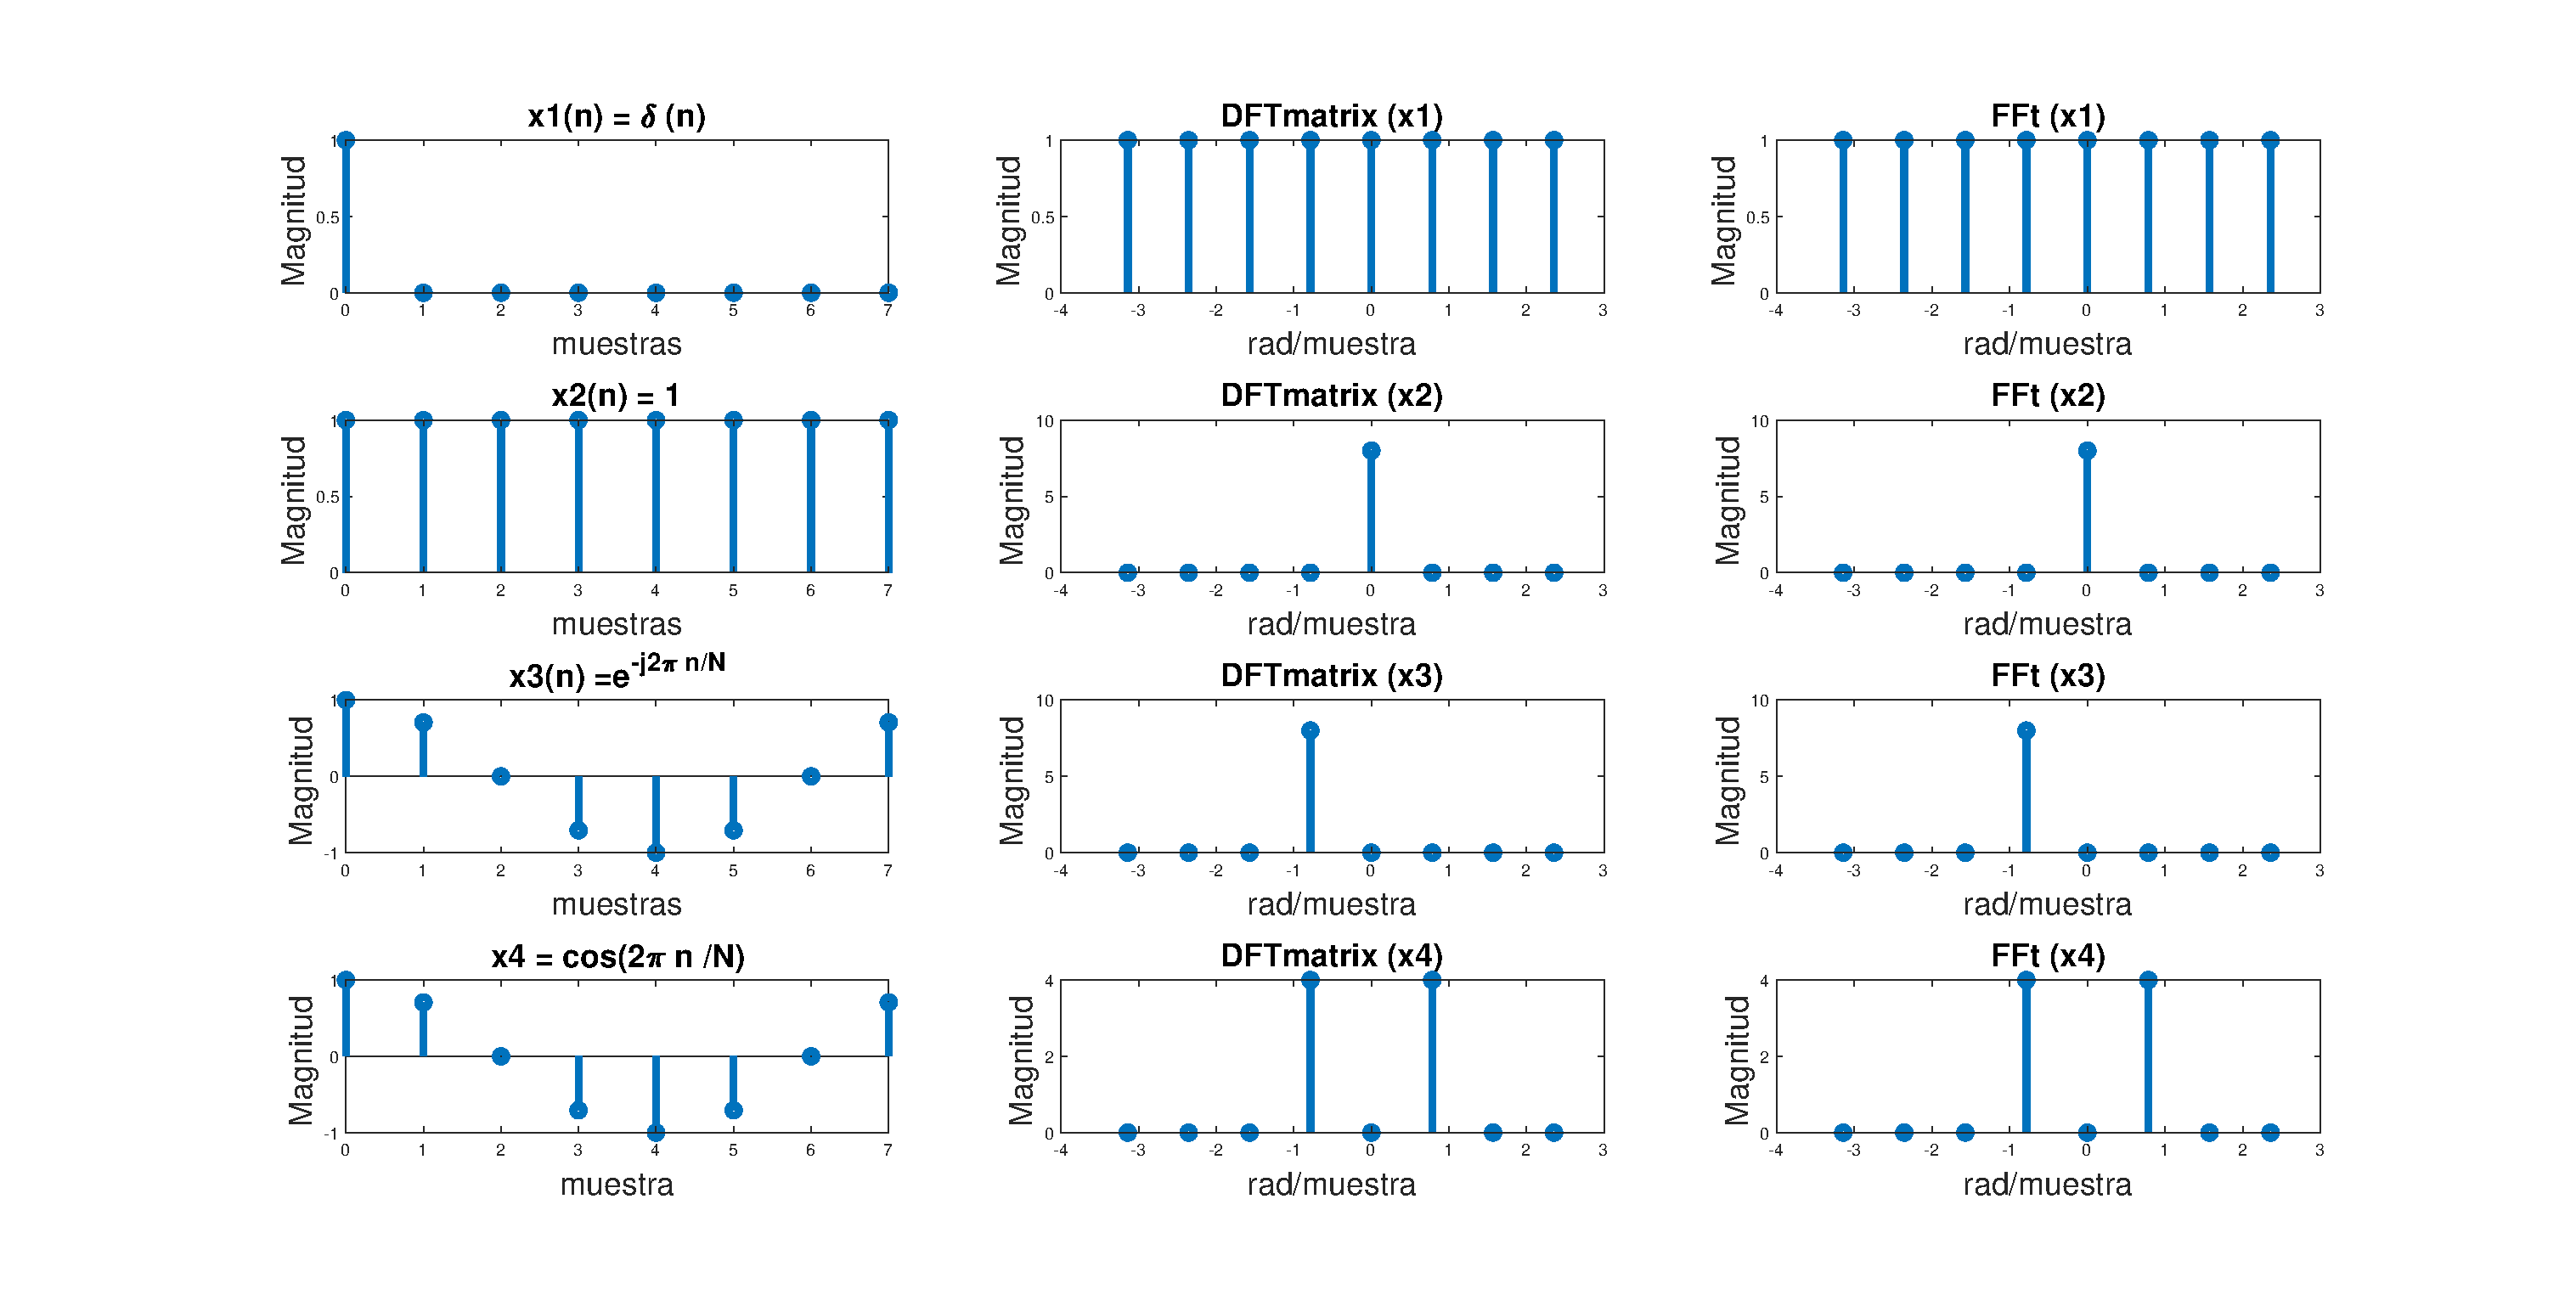
\includegraphics[scale = 0.3]{Figuras/p4_1-DFTmatrix.eps}
        \caption{Señales $x_1$, $x_2$, $x_3$ y $x_4$ generadas junto a sus respectivas DFT obtenida con la función implementada y FFT obtenida con comandos en MATLAB}
        \label{DFTmatrix}
    \end{figure}


Como se puede apreciar en las gráficas, al igual que en el caso anterior con la función \texttt{DFTsum(x)}, esta vez para la función \texttt{DFTmatrix(x)} se obtienen resultados cualitativamente idénticos a los que se obtienen haciendo uso del comando \textit{fft} de MATLAB. Cabe mencionar que nuevamente para el caso de la señal $x_3$ se ha graficado unicamente la parte real correspondiente.

A continuación se presenta una tabla con los errores cuadráticos medios asociados a ambas funciones implementadas que homologan el comportamiento del comando \textit{fft} de MATLAB.


  
 
 \begin{table}[H]
        \centering
        \begin{tabular}{|c|c|c|}
        \hline
         Señal    & MSE DFTsum $v/s$ fft & MSE DFTmatrix $v/s$ fft  \\
         \hline
         $x_1(n) = \delta (n)$   & $0$ & $0$ \\
         \hline
          $x_2(n) = 1$   &   $1.2195\cdot 10^{-30}$  & $3.8323\cdot 10^{-30}$\\
         \hline
            $ x_3(n) =e^{-j2 \pi n /N}$ &   $7.1631\cdot 10^{-31} $ & $3.8254\cdot 10^{-30}$  \\
         \hline
        
         $ x_4(n) = cos(2\pi n /N)$  &    $3.1880\cdot 10{-31}  $ & $5.9170\cdot 10^{-31}$\\
         \hline


        \end{tabular}
        \caption{Cuadro resumen para el error cuadrático medio entre el resultado de las funciones \texttt{DFTsum} y  \texttt{DFTmatrix} con respecto al resultado entregado por el comando \texttt{fft} de MATLAB para cada señal de prueba.}
        \label{MSE}
    \end{table}
    
    Todos los errores encontrados son despreciables ya que su orden de magnitud no es significativo respecto a las magnitudes con las que se trabaja en el contexto actual.
    

    %5.4
    \item Se utiliza el comando \texttt{timeit} de MATLAB para medir el tiempo de procesamiento de los métodos $fft, DFTsum$ y $dftmtx$, considerando $N = (100:100:5000)$ puntos.   
    
    Se grafica el tiempo de procesamiento para los valores de $N$, donde se escoge escala logarítmica para fines comparativo. El gráfico se muestra en la figura \ref{fig:p5_4cmp}. 
    
    \begin{figure}[H]
        \centering
        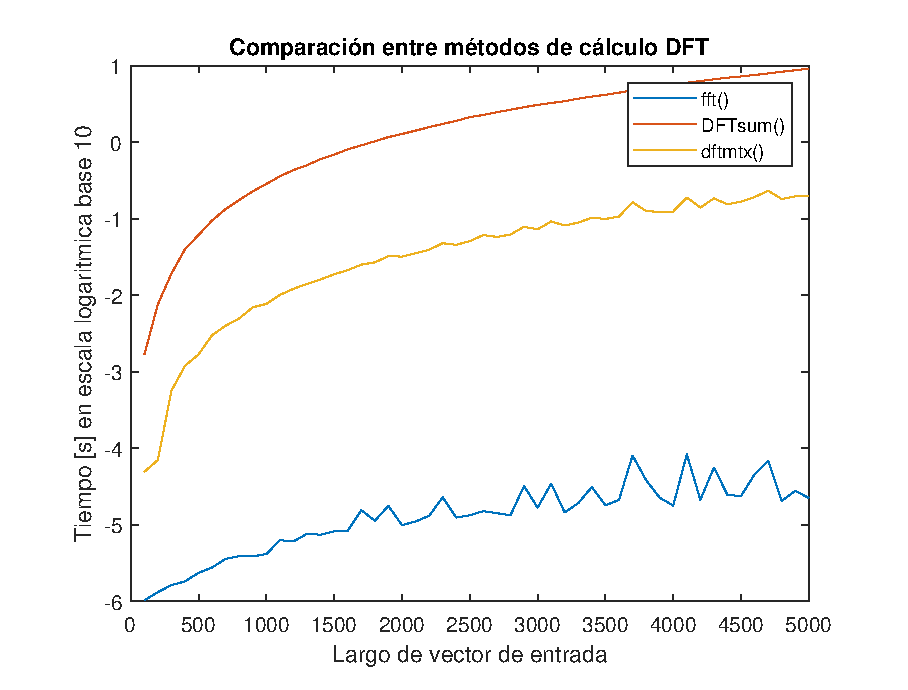
\includegraphics[width = .8\linewidth]{Figuras/p5_4cmp.eps}
        \caption{Tiempo de procesamiento para funciones $fft, DFTsum$ y $dftmtx$, considerando $N = (100:100:5000)$ puntos.}
        \label{fig:p5_4cmp}
    \end{figure}
    
    Con respecto al tiempo de procesamiento se concluye que:
    \begin{itemize}
        \item Para los largos probados de entrada, la $fft$ resulta más rápida que el método $dftmtx$ y este a su vez que el $DFTmtx$.
        \item La razón del tiempo de procesamiento entre $DFTsum$ y $fft$ es de aproximadamente $10^{-6}$, a partir de largos de 1000 muestras. Antes de las 1000 muestras la razón va en ascenso
        \item La razón del tiempo de procesamiento entre $DFTsum$ y $fft$ es de aproximadamente $10^{-4}$, a partir de largos de 1000 muestras.  Antes de las 1000 muestras la razón va en ascenso.
        \item La La razón del tiempo de procesamiento entre $DFTsum$ y $dftmtx$ es aproximadamente $10^{-2}$, para todos los largos de datos probados.
    \end{itemize}
    
    Con respecto a la memoria utilizada, claramente el método $dftmtx$ es el que ocupa más debido a que gerena la matriz de transformación que termina siendo de $N\times N$
    
    

    


    
    \end{enumerate} 
    




\newpage
\section{Algoritmo Radix-2 de la FFT}
\begin{enumerate}
\item Se experimenta con lograr la FFT con solo una reducción de orden. Para lo anterior se escribe la función $X = DFTdc(x)$, la cual implementa una etapa del algoritmo recursivo de la FFT y luego utiliza la función $DFTsum$ para obtener la DFT de las señales de muestras pares e impares.

El código escrito para la función $DFTdc$ se muestra a continuación:
\begin{lstlisting}[language = octave]
function X = DFTdc(x)
    N  = length(x);
    W  = exp(-1j*2*pi/N);
    Wk = W.^(0:(N/2-1));
    
    x0 = zeros(1,N/2);
    x1 = zeros(1,N/2);
    
    for i = 1:N/2
        x0(i) = x(2*i-1); %OBS "par"   1,3,5,... en MATLAB
        x1(i) = x(2*i);   %OBS "impar" 2,4,6,... en MATLAB       
    end
    
    X0 = DFTsum(x0); X1 = DFTsum(x1);
    
    X_izq = X0 + Wk.*X1;
    X_der = X0 - Wk.*X1;
    
    X = [X_izq X_der];    
end
\end{lstlisting}

Posteriormente se utiliza la función generada para obtener la DFT de 3 señales de prueba:
\begin{itemize}
    \item Señal a: $x(n) = \delta(n)$
    \item Señal b: $x(n) = 1$
    \item Señal c: $x(n) = e^{-j\frac{2\pi n}{8}}$
\end{itemize}

Las magnitudes de la DFT obtenidas con la función para las señales de prueba se muestran en la figura \ref{p6_1dft}, donde además se muestran las magnitudes de la DFT utilizando el comando $fft$ de MATLAB con fines comparativos. Como era de esperarse, no se aprecian diferencias visuales en los resultados obtenidos.

\begin{figure}[H]
    \centering
    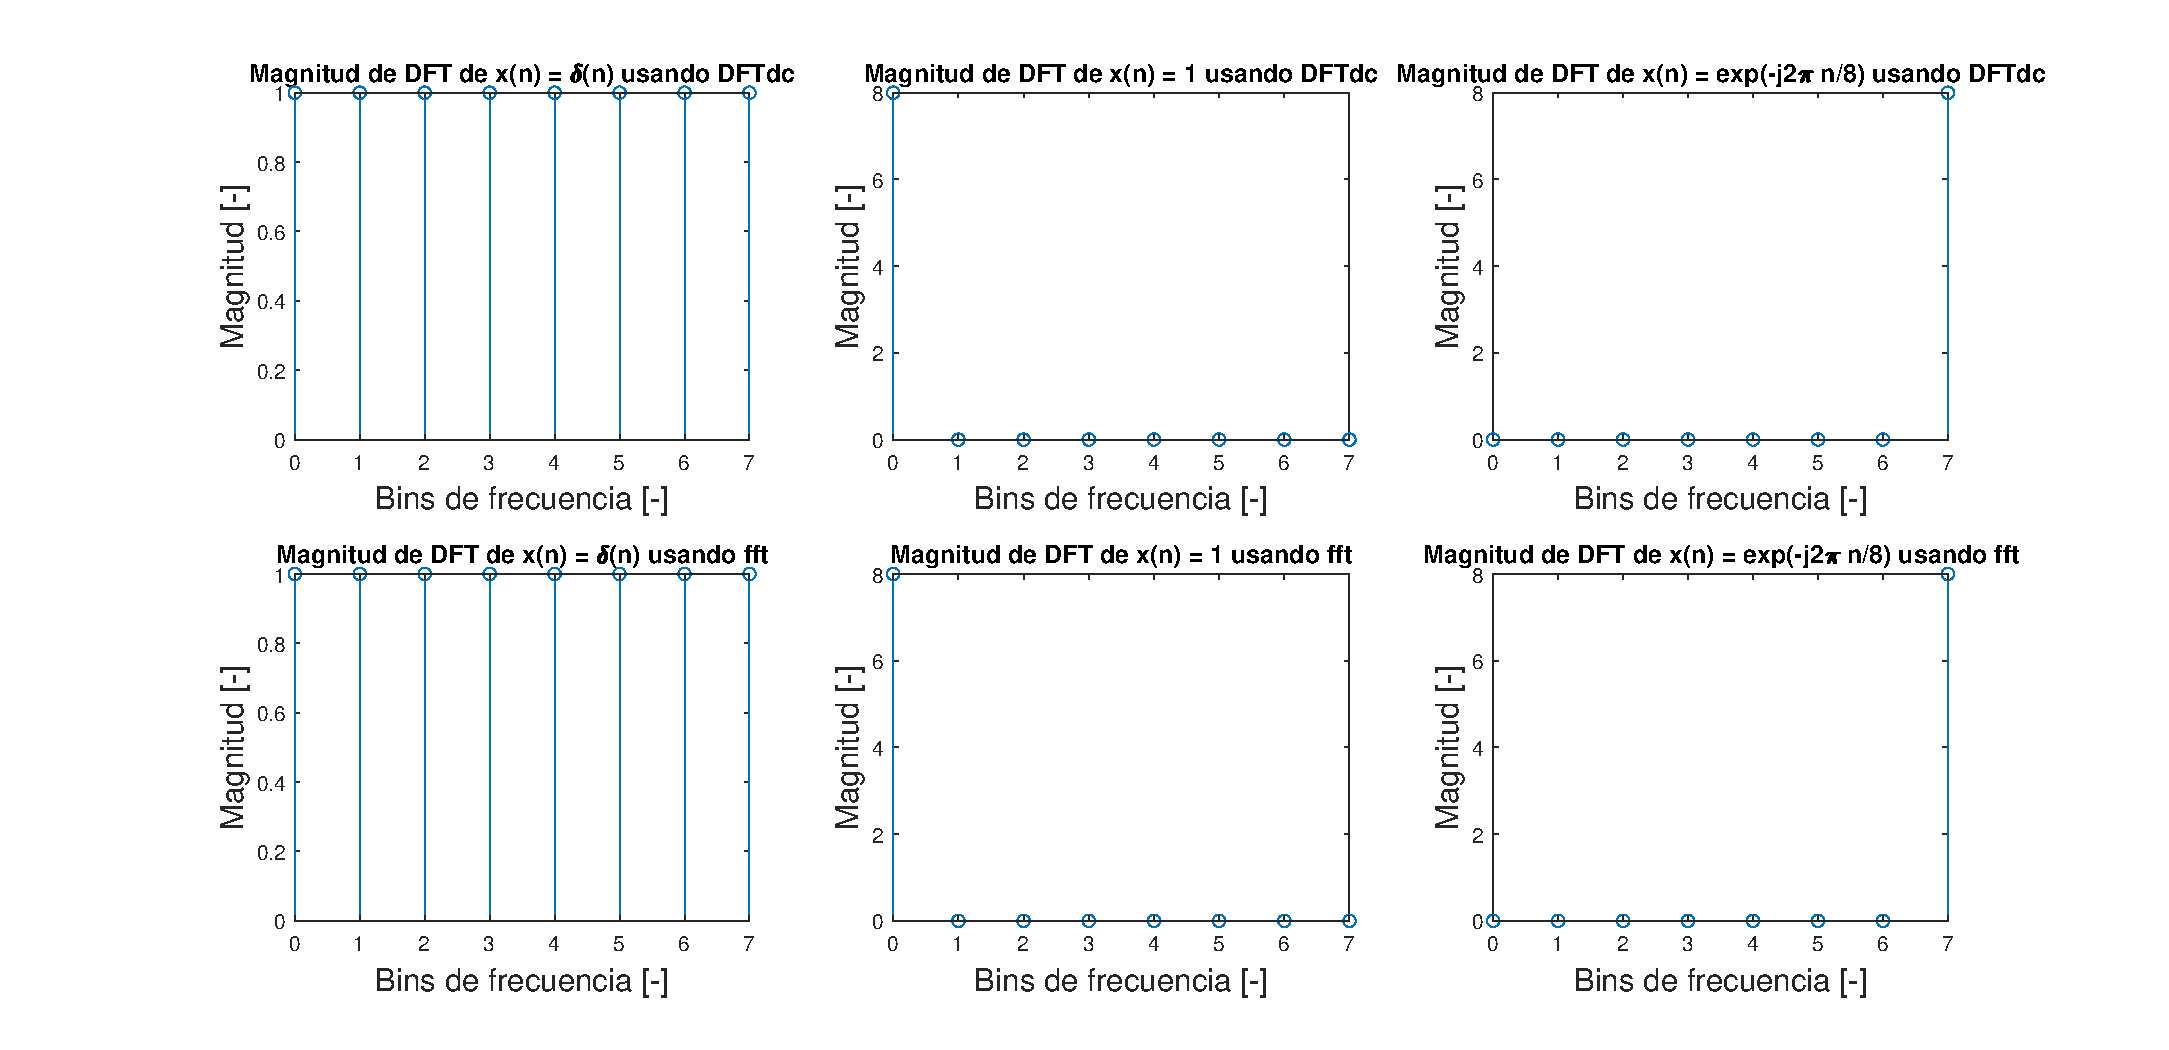
\includegraphics[width = .98 \linewidth]{Figuras/p6_1dft.eps}
    \caption{Comparación entre magnitudes de DFT obtenidas con función $DFTdc$ y $fft$ en MATLAB.}
    \label{p6_1dft}
\end{figure}

Finalmente se obtiene el tiempo de procesamiento para la función $DFTdc$ y $fft$, obteniendo:
\begin{itemize}
    \item $DFTdc$: $3.64123\cdot 10^{-5}~s$ 
    \item $fft$:   $9.84100\cdot 10^{-7}~s$
\end{itemize}
Se aprecia que la implementación de la $fft$ de MATLAB es muy superior a la función generada al calcular una DFT de 8 puntos.

\item Se experimenta con FFTs de 2, 4 y 8 puntos, programando las funciones $FFT2, FFT4$ y $FFT8$, las cuales corresponden a implementaciones explícitas de las ecuaciones del algoritmo fft.

En primer lugar se implementa la función $FFT2$, a partir de las ecuaciones:
\begin{align*}
    X^{(2)}(0) &= x(0) + x(1)\\
    X^{(2)}(1) &= x(0) - x(1)
\end{align*}
Donde $X^{(2)}$ corresponde a la DFT de la señal $x$, la cual tiene 2 puntos.

El código escrito para la función $FFT2$ se muestra a continuación:
\begin{lstlisting}[language = octave]
function X = FFT2(x)
    X = zeros(1,2);
    
    X(1) = x(1) + x(2);
    X(2) = x(1) - x(2);
end
\end{lstlisting}

Las funciones $FFT4$ y $FFT8$, corresponden a la implementación con $N=4$ y $8$ respectivamente de las siguientes ecuaciones:
\begin{align*}
    X^{(N)}(k)   &= X_0^{(N/2)}(k) + W^k_N X_1^{(N/2)}(k)\\
    X^{(N)}(N/2+k) &= X_0^{(N/2)}(N/2+k) - W^k_N X_1^{(N/2)}(N/2+k)
\end{align*}
Donde
\begin{itemize}
    \item $X^{(N)}$ corresponde a la DFT de la señal $x$, la cual tiene $N$ puntos 
    \item $X_0^{(N/2)}(k)$ y $X_0^{(N/2)}(k)$ corresponden a la DFT de la señal de muestras pares e impares de $x$.
    \item $W_N = e^{(-j2\pi/N)}$ corresponde al factor de twiddle.
\end{itemize}

La implementación de $FFT4$, se muestra a continuación:
\begin{lstlisting}[language = octave]
function X = FFT4(x)
    X = zeros(1,4);
    
    x0 = [x(1) x(3)]; %Muestras "pares"
    x1 = [x(2) x(4)]; %Muestras "impares"
    
    X0 = FFT2(x0);
    X1 = FFT2(x1);
    
    X(1) = X0(1) +   (1)*X1(1);
    X(2) = X0(2) + (-1j)*X1(2);    
    
    X(3) = X0(1) -   (1)*X1(1);
    X(4) = X0(2) - (-1j)*X1(2);    
end
\end{lstlisting}

La implementación de $FFT8$ se muestra a continuación:
\begin{lstlisting}[language = octave]
function X = FFT8(x)
    X = zeros(1,8);
    
    x0 = [x(1) x(3) x(5) x(7)]; %Muestras "pares"
    x1 = [x(2) x(4) x(6) x(8)]; %Muestras "impares"
    
    X0 = FFT4(x0);
    X1 = FFT4(x1);
    
    X(1) = X0(1) +               (1)*X1(1);
    X(2) = X0(2) +   (exp(-1j*pi/4))*X1(2);
    X(3) = X0(3) +             (-1j)*X1(3);
    X(4) = X0(4) + (exp(-1j*3*pi/4))*X1(4);
    
    X(5) = X0(1) -               (1)*X1(1);
    X(6) = X0(2) -   (exp(-1j*pi/4))*X1(2);
    X(7) = X0(3) -             (-1j)*X1(3);
    X(8) = X0(4) - (exp(-1j*3*pi/4))*X1(4);
end
\end{lstlisting}

Posteriormente se utiliza la función $FFT8$ generada para obtener la DFT de 3 señales de prueba del punto anterior.

Las magnitudes de la DFT obtenidas con la función para las señales de prueba se muestran en la figura \ref{p6_2dft}, donde además se muestran las magnitudes de la DFT utilizando el comando $fft$ de MATLAB con fines comparativos. Como era de esperarse, no se aprecian diferencias visuales en los resultados obtenidos.

\begin{figure}[H]
    \centering
    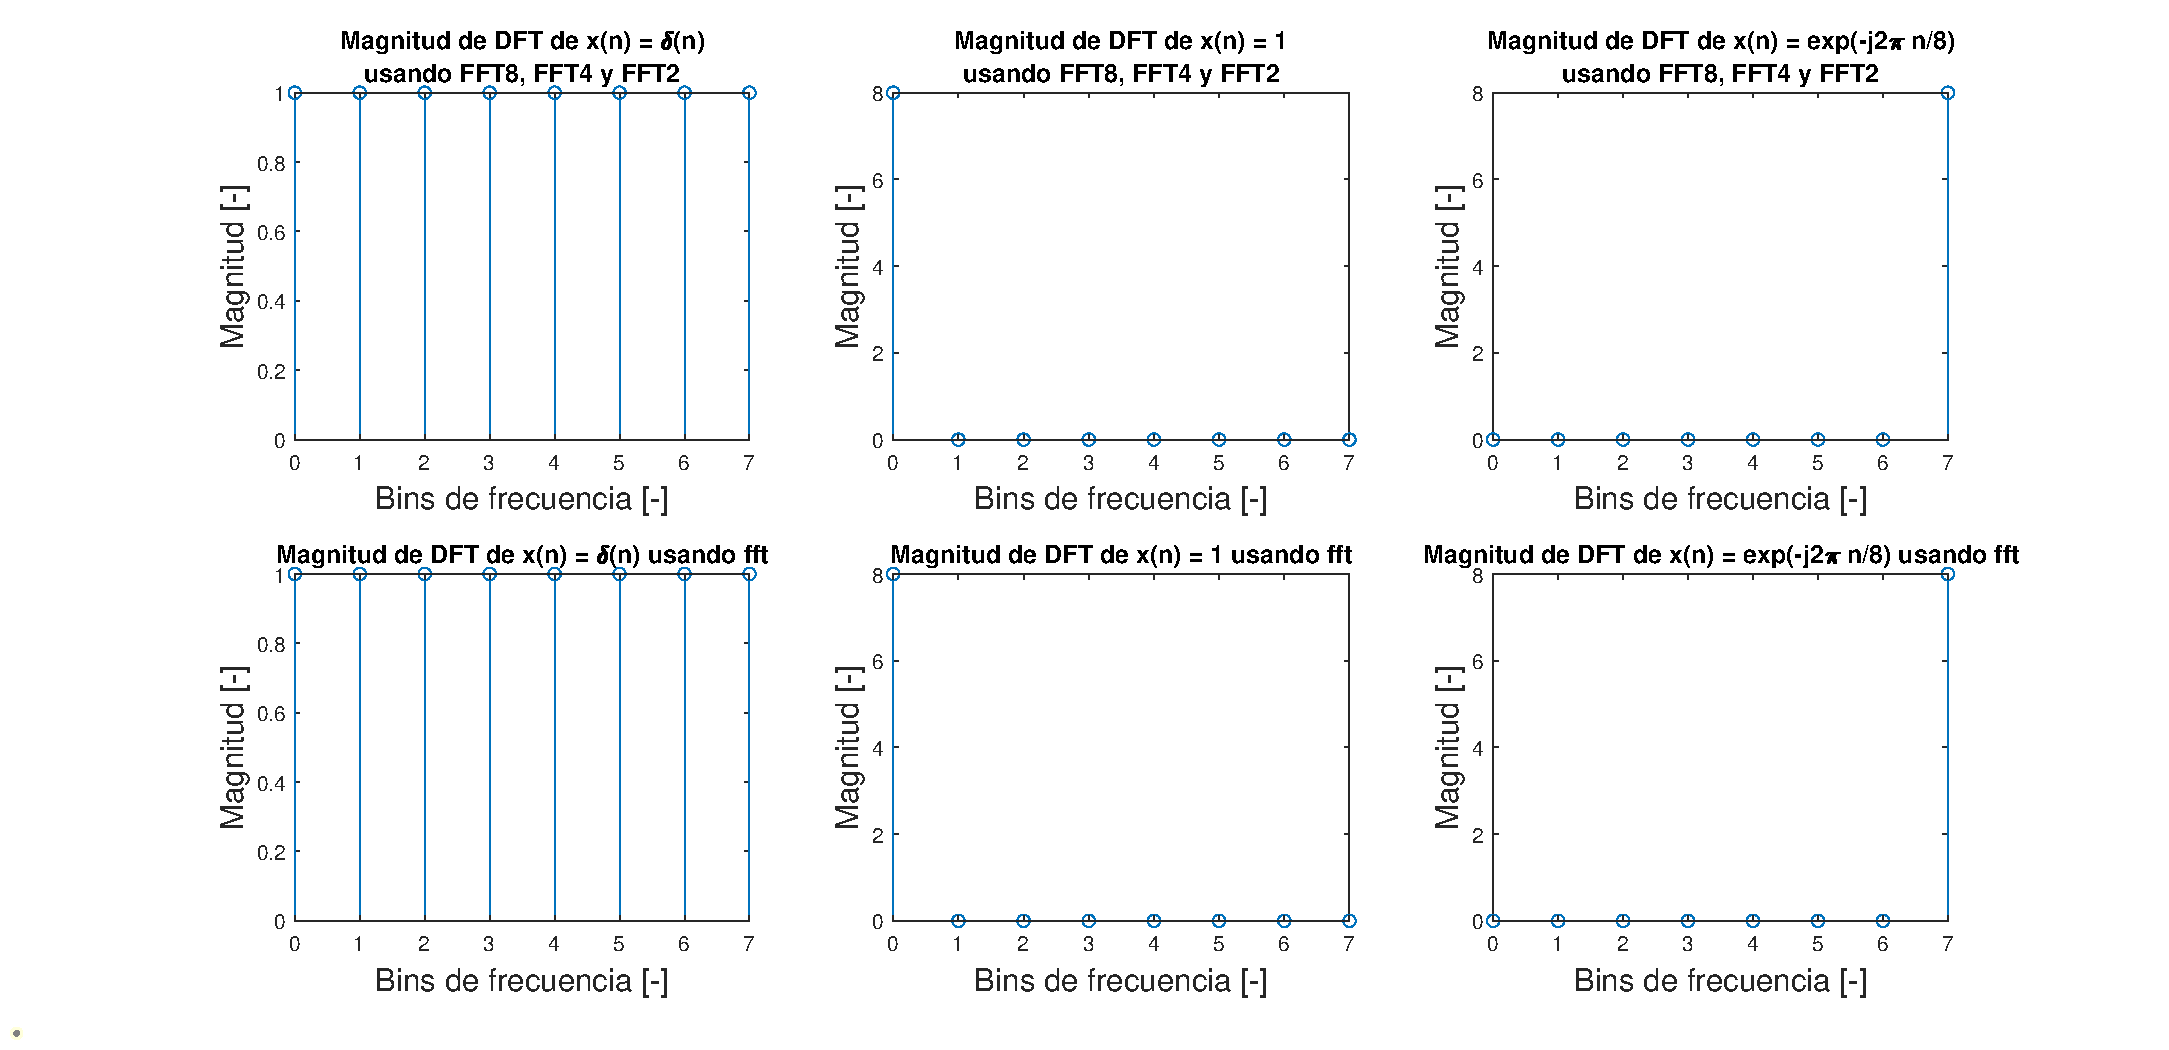
\includegraphics[width = .98 \linewidth]{Figuras/p6_2dft.eps}
    \caption{Comparación entre magnitudes de DFT obtenidas con función $FFT8$ y $fft$ en MATLAB.}
    \label{p6_2dft}
\end{figure}

Finalmente se obtiene el tiempo de procesamiento para la función $FFT8$ y $fft$, obteniendo:
\begin{itemize}
    \item $FFT8$: $1.63822\cdot 10^{-5}~s$ %3.64123e-05 seg 
    \item $fft$:  $7.75409\cdot 10^{-7}~s$ %9.84100e-07 seg
\end{itemize}
Se aprecia que la implementación de la $fft$ de MATLAB sigue siendo muy superior a la función generada al calcular una DFT de 8 puntos. Sin embargo, cabe destacar que hubo una mejora con respecto al algoritmo $DFTdc$.

\item Se crea la función recursiva $X = fft\_stage(x)$, la cual aplica el algoritmo FFT para señales de largo $2^{n}$. El código se muestra a continuación:

\begin{lstlisting}
function X = fft_stage(x)
    N = length(x);
    
    if (N == 2)
        X = FFT2(x);
        return
    else    
        x0    = zeros(1,N/2); x1    = zeros(1,N/2);        
    
        for i = 1:N/2
            x0(i) = x(2*i-1); %OBS "par"   1,3,... en MATLAB
            x1(i) = x(2*i);   %OBS "impar" 2,4,... en MATLAB       
        end
    
        W = exp(-1j*2*pi/N);  Wk = W.^(0:(N/2-1));        
        X0 = fft_stage(x0) ;  X1 = fft_stage(x1) ; 
    
        X_izq = X0 + Wk.*X1;
        X_der = X0 - Wk.*X1;
    
        X = [X_izq X_der];
    end
end
\end{lstlisting}

Se utiliza el comando \texttt{timeit} de MATLAB para comparar el tiempo de procesamiento al utilizar de entrada la señal del punto \textbf{4.3}, considerando largos de $N = [2^{10}, 2^{11}, \dots , 2^{19}]$. Los gráficos con los tiempos de cómputo se muestran en la figura \ref{p6_3cmp}
\begin{figure}[H]
    \centering
    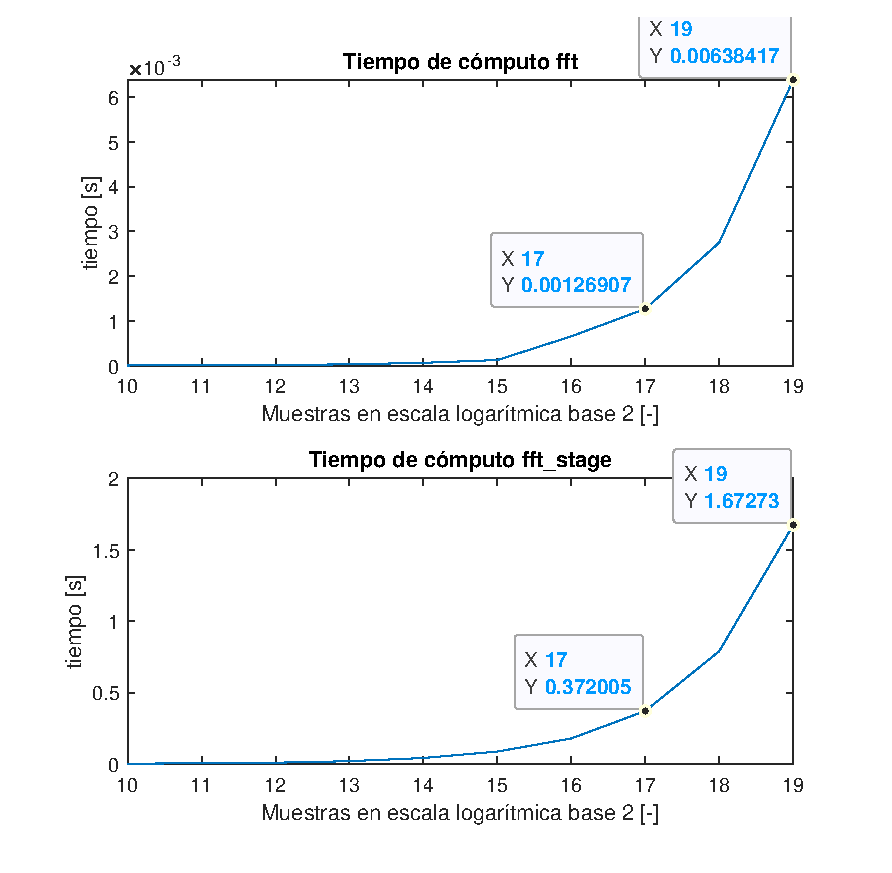
\includegraphics[width = .98 \linewidth]{Figuras/p6_3_cmp.eps}
    \caption{Tiempos de cómputo de función $fft\_stage$ y $fft$ para distintos largos de señal.}
    \label{p6_3cmp}
\end{figure}

De los resultados de tiempo de cómputo obtenidos se concluye que:
\begin{itemize}
    \item La implementación de MATLAB es muy superior a $fft\_stage$. La razón entre el tiempo de cómputo de la $fft$ con respecto a $fft\_stage$ es del orden de $10^-3$. 
    \item La curva de tiempo de cómputo en ambos algoritmos son similares.
\end{itemize}
\end{enumerate}

\newpage
\section{Algoritmo Goertzel }
Se busca poder realizar una implementación del \textit{algoritmo de Goertzel} en lenguaje C mediante el uso de \textit{S-Function} en MATLAB trabajando sobre el proyecto entregado como material de apoyo para la experiencia del laboratorio.


\begin{enumerate}
    \item Se crea la función \textit{computeGoertzel()} que recibe como argumentos el puntero al estado del filtro Goertzel y una muestra de entrada con el código que se muestra a continuación
    
    \begin{lstlisting}[language = C]
static double computeGoertzel(goertzelState_t *state,
                            double filterInput)

//Incrementa contador
	state->samplesCounter += 1;
//IIR
state->outputs[2] = state->outputs[1];
state->outputs[1] = state->outputs[0];
state->outputs[0] = filterInput + 
                    (state->A1)*state->outputs[1] 
                    - state->outputs[2];

//FIR
  if (GOERTZEL_N <= state->samplesCounter){
    state->binReal = state->cosW*state->outputs[1] 
                    - state->outputs[2];
    state->binImag = state->sinW*state->outputs[1];
    state->binMag = sqrt((state->binReal*state->binReal) 
                        +(state->binImag*state->binImag)  ); 

    resetGoertzel(state);
  }

	return state->binMag;
}

    \end{lstlisting}
    
    
    Otras funciones relevantes en el funcionamiento del algoritmo de Groetzel son aquellas que inicializan y reinician  los estados del filtro. La función \texttt{initGoertzel()} encargada de la inicialización se muestra a continuación, mientras que la función \texttt{resetGoertzel} solo reestablece en cero los valores del vector de salidas y el contador de muestras presentes en la estructura entregada para el laboratorio.
    
    \begin{lstlisting}[language = C]
static void initGoertzel(goertzelState_t *state, 
                        uint64_t kFrequency)
{
  state->samplesCounter 	= 0;
  state->cosW = cos(2*M_PI*kFrequency/GOERTZEL_N);
  state->sinW = sin(2*M_PI*kFrequency/GOERTZEL_N);
  state->A1  = 2*cos(2*M_PI*kFrequency/GOERTZEL_N);

  state->outputs[0] = 0.0;
  state->outputs[1] = 0.0;
  state->outputs[2] = 0.0;

  state->binReal =0.0;
  state->binImag=0.0;
  state->binMag = 0.0;

  return;    }
    \end{lstlisting}
    
    
    
El algoritmo de Goertzel entrega la magnitud de bines específicos en el espectro de una señal de N muestras, para evaluar el correcto funcionamiento de la implementación hecha se utiliza el archivo de audio \textit{dtmfSequence\_16\_16.wav}, para el cual se obtiene la DFT para los primeros 256 valores con el comando de MATLAB \textit{fft} y luego se grafica indicando el valor que resulta en los bines 8,9 y 10.  Por otro lado se simula el algoritmo con simulink y se analiza la primera muestra ( definida por los 256 primeros datos del archivo de audio) y se compara la magnitud presente en el gráfico de la DFT con la magnitud obtenida mediante simulación.

\begin{figure}[H]
    \centering
    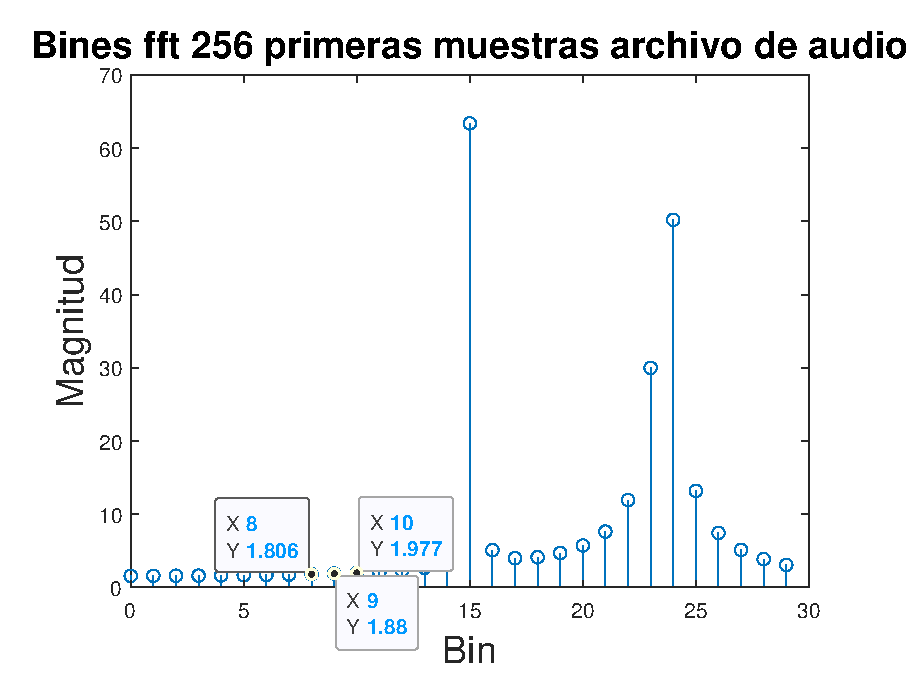
\includegraphics[width = .8 \linewidth]{Figuras/p7_1-fft_dtmf.eps}
    \caption{Gráfica de los bines obtenidos por la fft de las primeras 256 muestras del archivo de audio \textit{dtmfSequence\_16\_16.wav}.}
    \label{fft_256}
\end{figure}

\begin{figure}[H]
    \centering
    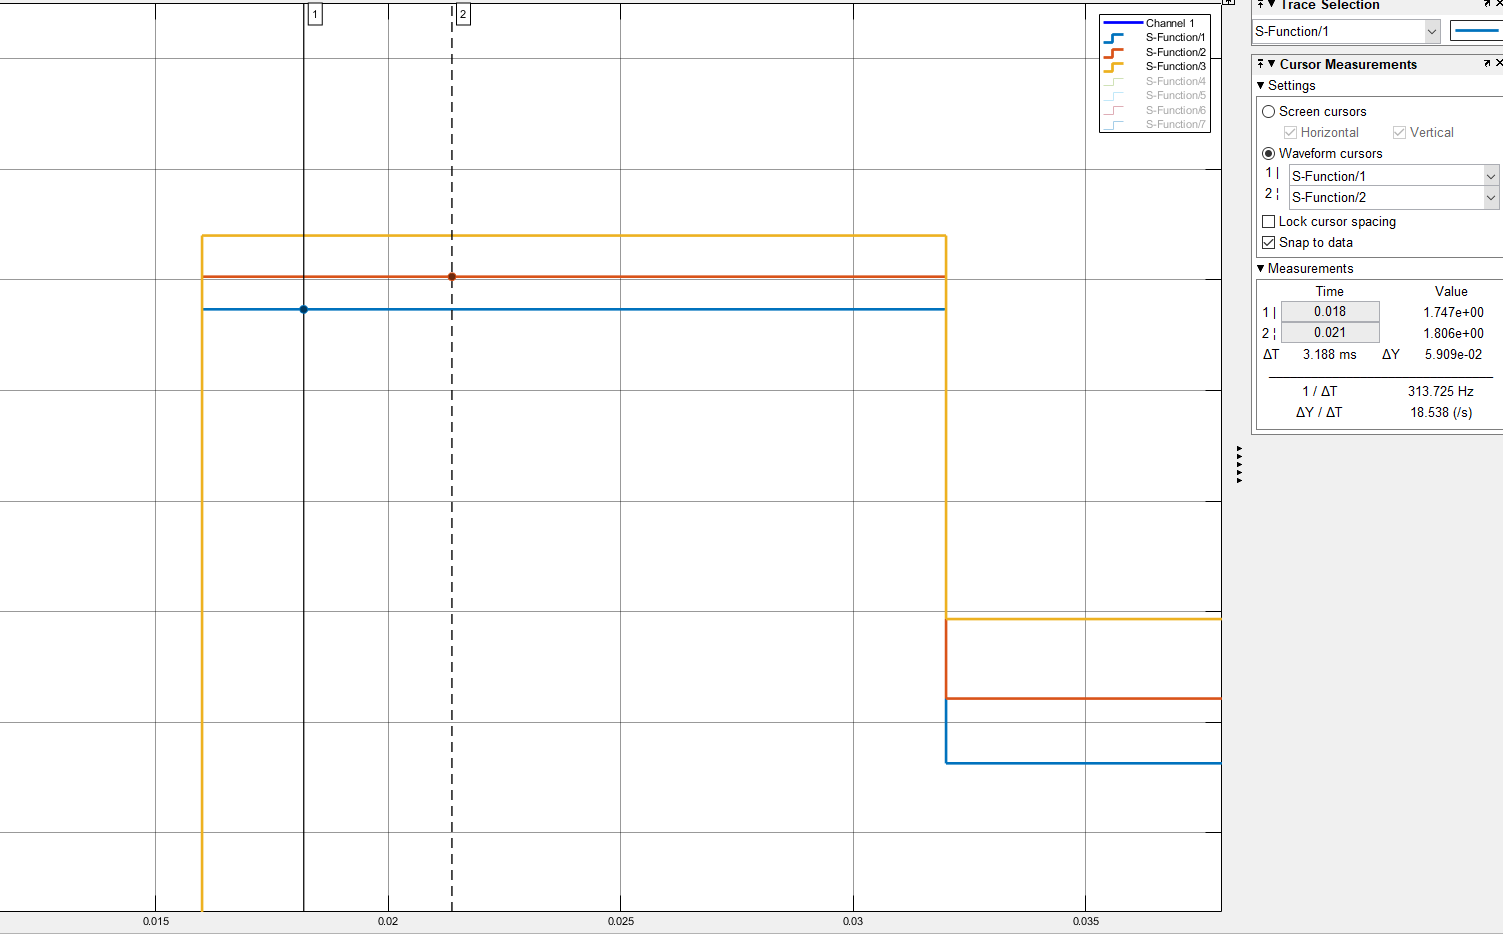
\includegraphics[scale = 0.4]{Figuras/7_1-mag-Goertzel.png}
    \caption{Magnitud de los bines 8, 9 y 10 asociados al archivo de audio  \textit{dtmfSequence\_16\_16.wav}, obtenidas mediante simulación.}
    \label{gotze_256}
\end{figure}


En la última figura las leyendas \textit{S-Function/1}, \textit{S-Function/2} y \textit{S-Function/3} corresponden a las magnitudes de los bines 8, 9 y 10 respectivamente. Comparando los valores que se muestran en el cuadro de datos a la derecha con los valores que indican los cuadros \textit{data tip} para los bines 8, 9 y 10 se puede ver que coinciden por lo que se concluye que la implementación del algoritmo de Goertzel funciona de manera correcta.


\item   Se instancia un total de 7 filtro Goertzel para lograr obtener los bins de frecuencia más cercanos a las frecuencias de los DTMF de la experiencia anterior, considerando el mismo archivo de usado anteriormente, el cual posee una frecuencia de muestreo de $16~ksps$ y nuevamente se analizan una cantidad N = 256 de muestras.

Para escoger correctamente los $k$ bins correspondiente a cada frecuencia DTMF se usa la expresión 

$$ k-Bin =  \frac{f_{DTMF} \cdot N}{Fs}$$ 

Redondeando de ser necesario el resultado, pues los $k- bines$ han de ser números enteros. De esta forma se obtiene la siguiente tabla



 \begin{table}[H]
        \centering
        \begin{tabular}{|c|c|}
        \hline
         frecuencia DTMF   & k-Bin  \\
         \hline
697  Hz & 11 \\
\hline
770  Hz & 12 \\
\hline
 852  Hz & 14\\
\hline

941  Hz & 15\\
\hline


1209  Hz & 19\\
\hline
 
941  Hz & 15\\
\hline
 
1336 Hz & 21\\
\hline

1336 Hz & 21\\
\hline

        \end{tabular}
        \caption{Cuadro resumen para el error cuadrático medio entre el resultado de la función \texttt{DFTsum} y el resultado entregado por el comando \texttt{fft} de MATLAB para cada señal de prueba.}
        \label{MSE}
    \end{table}
    
    
Se modifica la sección de código correspondiente quedando de la siguiente forma 

\begin{lstlisting}
 #define GOERTZEL1_K_BIN	    (11)
 #define GOERTZEL2_K_BIN	    (12)
 #define GOERTZEL3_K_BIN	    (14)
 #define GOERTZEL4_K_BIN	    (15)
 #define GOERTZEL5_K_BIN	    (19)
 #define GOERTZEL6_K_BIN	    (21)
 #define GOERTZEL7_K_BIN	    (24)
\end{lstlisting}


Usando los comandos \textit{subplot} y \textit{bar} se grafican los resultados para las 7 salidas de los filtros Goertzel, y tal como se esperaba, se cumple que en todo momento existen solo dos de las 7 componentes (bines) con magnitudes altas , correspondientes a las frfecuencias DTMF. Esta gráfica se muestra en la figrua \ref{dtmf}

\begin{figure}[H]
    \centering
    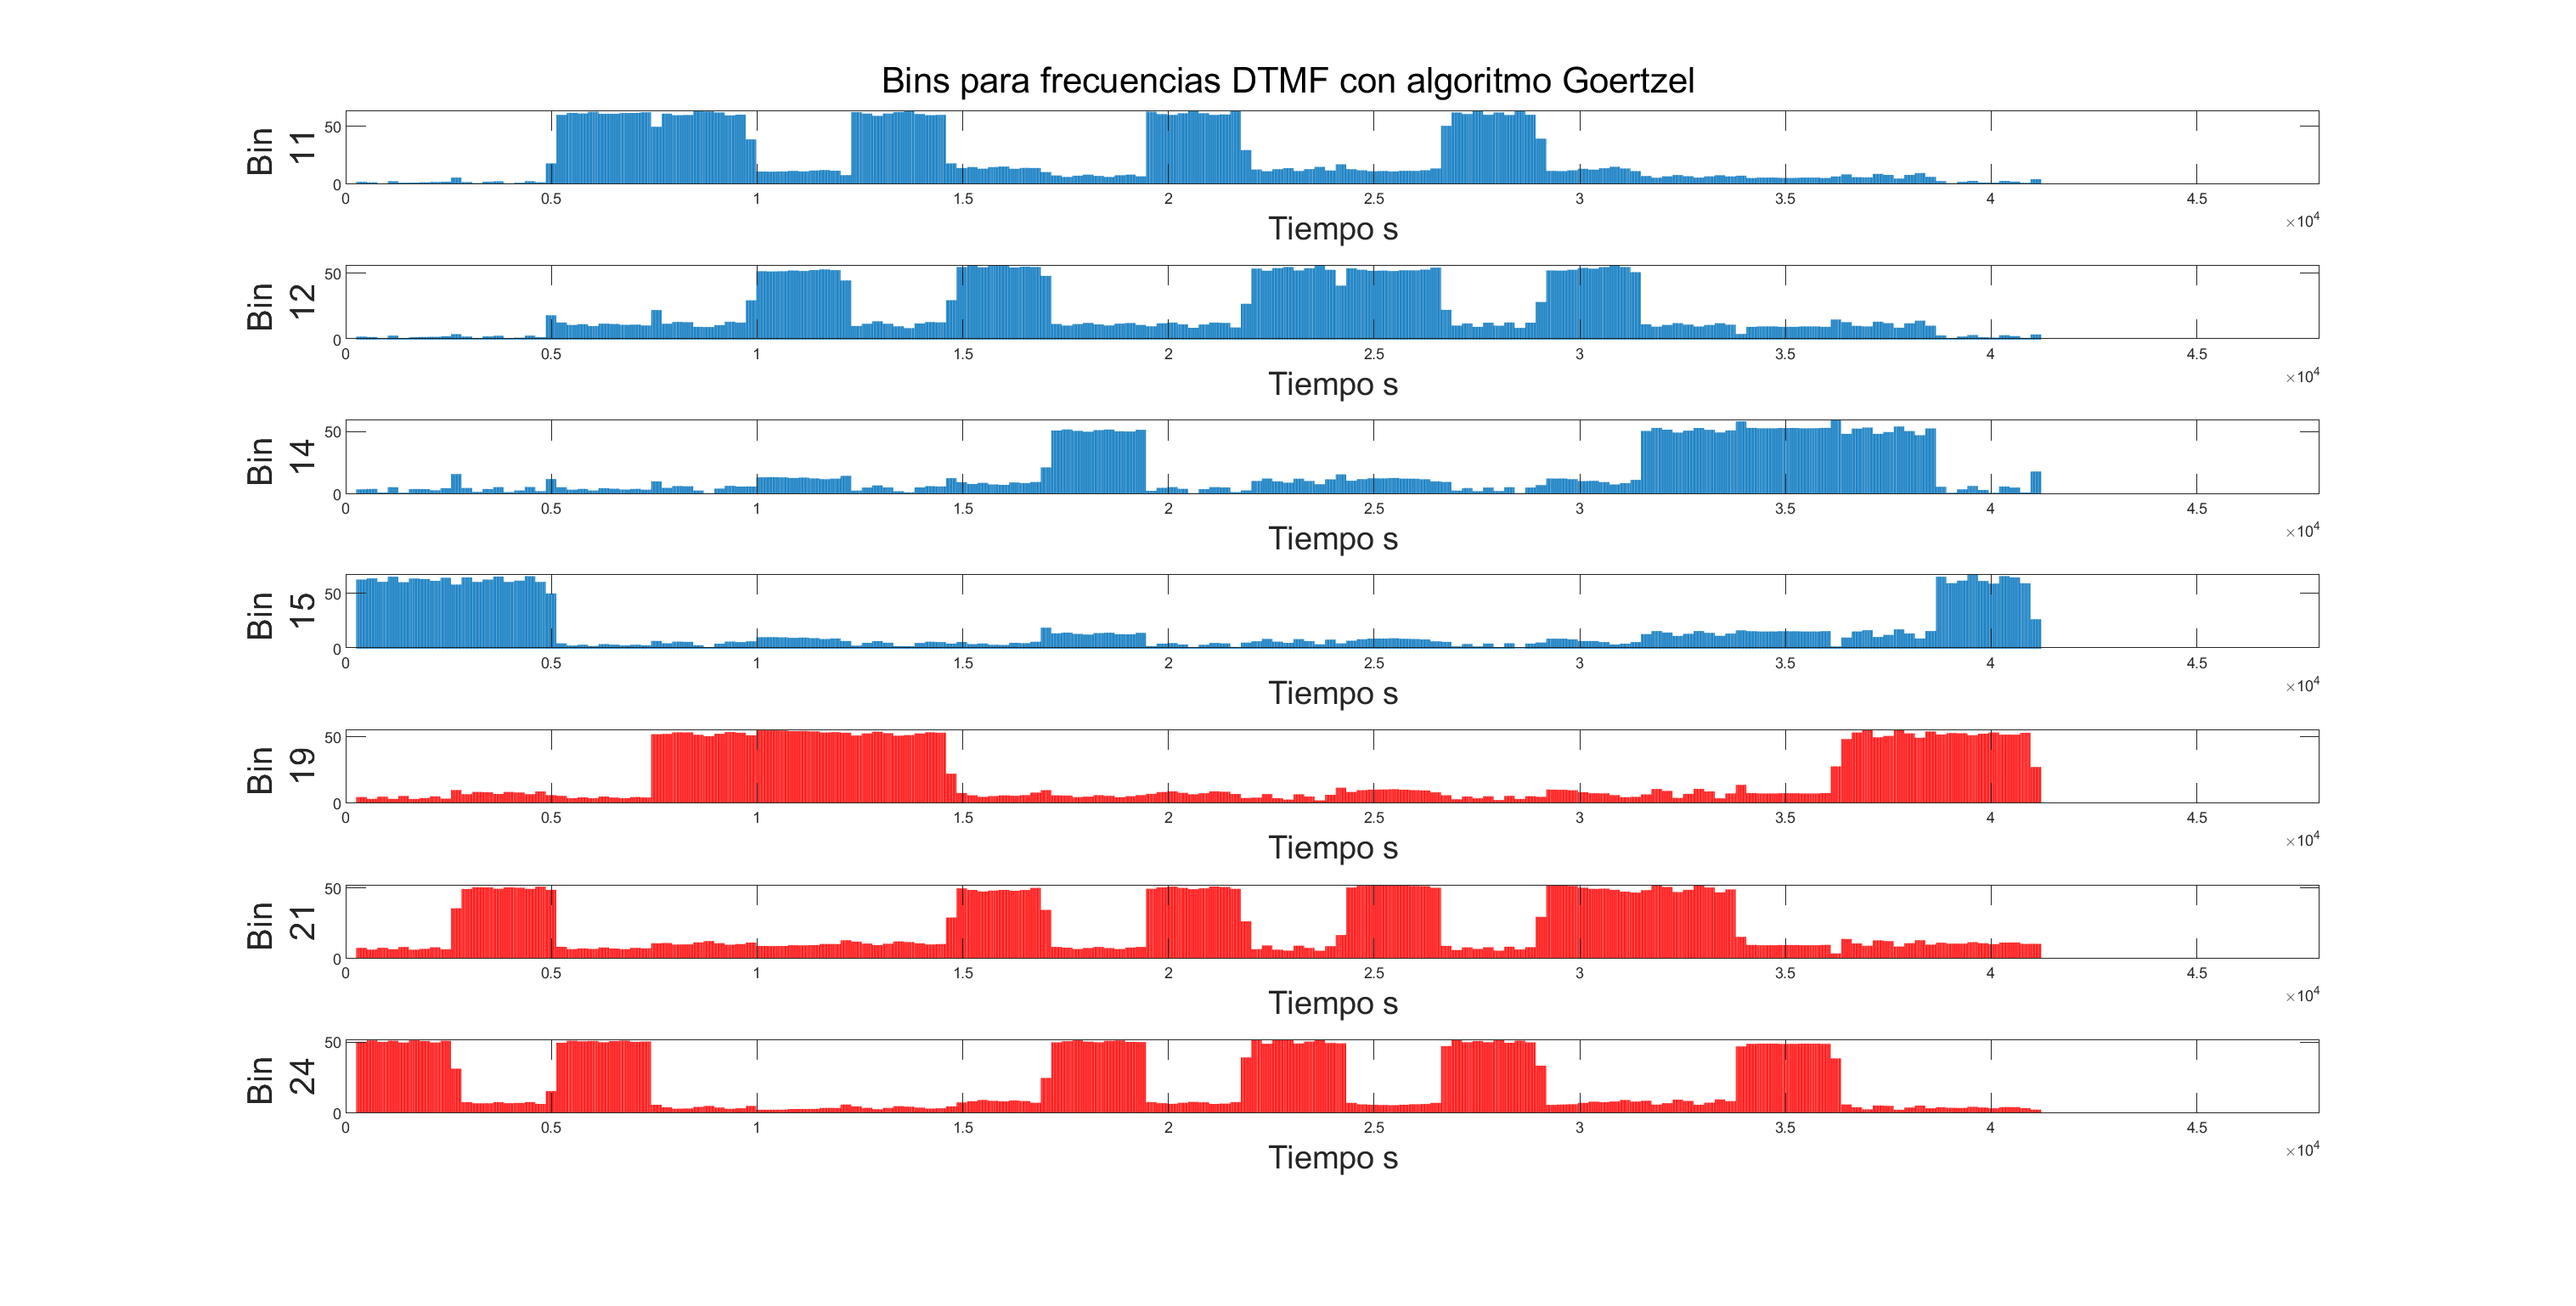
\includegraphics[scale = 0.35]{Figuras/p7_2.eps}
    \caption{Bins asociados a las frecuencias DTMF graficados en el tiempo usando el algoritmo de Goertzel}
    \label{dtmf}
\end{figure}

\end{enumerate}

  
  
  
  

  












\end{document}

